\documentclass[11pt,fleqn]{book} % Default font size and left-justified equations

%%%%%%%%%%%%%%%%%%%%%%%%%%%%%%%%%%%%%%%%%
% The Legrand Orange Book
% Structural Definitions File
% Version 2.1 (26/09/2018)
%
% Original author:
% Mathias Legrand (legrand.mathias@gmail.com) with modifications by:
% Vel (vel@latextemplates.com)
% 
% This file was downloaded from:
% http://www.LaTeXTemplates.com
%
% License:
% CC BY-NC-SA 3.0 (http://creativecommons.org/licenses/by-nc-sa/3.0/)
%
%%%%%%%%%%%%%%%%%%%%%%%%%%%%%%%%%%%%%%%%%

%----------------------------------------------------------------------------------------
%	VARIOUS REQUIRED PACKAGES AND CONFIGURATIONS
%----------------------------------------------------------------------------------------

\usepackage[table]{xcolor}

\usepackage{graphicx}
\usepackage{tabularx} % Required for including pictures
\usepackage{pgf,tikz,tkz-tab,eurosym,yhmath, stmaryrd}
\usepackage{pgfplots}
\usepackage{mathrsfs}
\usetikzlibrary{patterns}
\usetikzlibrary{trees}
\graphicspath{{../../Pictures/}}
\usepackage{multicol} 


\usepackage[english]{babel} % English language/hyphenation
\usepackage{icomma}
\usepackage{enumitem} % Customize lists
\setlist{nolistsep, nosep, nolistsep} % Reduce spacing between bullet points and numbered lists

\usepackage{booktabs} % Required for nicer horizontal rules in tables

 % Required for specifying colors by name


\definecolor{ocre}{RGB}{243,102,25} % Define the orange color used for highlighting throughout the book

\usepackage{listings}

\definecolor{codegreen}{rgb}{0,0.6,0}
\definecolor{codegray}{rgb}{0.5,0.5,0.5}
\definecolor{codepurple}{rgb}{0.58,0,0.82}
\definecolor{backcolour}{rgb}{0.95,0.95,0.92}

\lstdefinestyle{mystyle}{
    backgroundcolor=\color{backcolour},   
    commentstyle=\color{codegreen},
    keywordstyle=\color{magenta},
    numberstyle=\tiny\color{codegray},
    stringstyle=\color{codepurple},
    basicstyle=\ttfamily\footnotesize,
    breakatwhitespace=false,         
    breaklines=true,                 
    captionpos=b,                    
    keepspaces=true,                 
    numbers=left,                    
    numbersep=5pt,                  
    showspaces=false,                
    showstringspaces=false,
    showtabs=false,                  
    tabsize=2
}

\lstset{style=mystyle}

%----------------------------------------------------------------------------------------
% Paramétrage XSIM
%----------------------------------------------------------------------------------------

\usepackage[no-files]{xsim}


\DeclareExerciseEnvironmentTemplate{myex}{%
    \textbf{%
      \hypertarget{ex:\ExerciseID}{\sffamily{\ensuremath{\blacktriangleright}} Exercice \GetExerciseProperty{counter} \GetExerciseProperty{subtitle} --}
      \hyperlink{sol:\ExerciseID}{Voir le corrigé}%
    }\par
}{\par\smallskip}

\DeclareExerciseEnvironmentTemplate{mysol}{%
    \textbf{%
      \hypertarget{sol:\ExerciseID}{\sffamily{\ensuremath{\blacktriangleright}} Correction \GetExerciseProperty{counter} --}
      \hyperlink{ex:\ExerciseID}{Voir l'énoncé}%
    }\par
}{\par\medskip}

\xsimsetup{
  exercise/template = myex ,
  solution/template = mysol 
}

%Collection exercices

\DeclareExerciseTagging{topic}

\xsimsetup{collect}

%----------------------------------------------------------------------------------------
% SYMBOLES
%----------------------------------------------------------------------------------------

\newcommand\imCMsym[4][\mathord]{%
  \DeclareFontFamily{U} {#2}{}
  \DeclareFontShape{U}{#2}{m}{n}{
    <-6> #25
    <6-7> #26
    <7-8> #27
    <8-9> #28
    <9-10> #29
    <10-12> #210
    <12-> #212}{}
  \DeclareSymbolFont{CM#2} {U} {#2}{m}{n}
  \DeclareMathSymbol{#4}{#1}{CM#2}{#3}
}
\newcommand\alsoimCMsym[4][\mathord]{\DeclareMathSymbol{#4}{#1}{CM#2}{#3}}

\imCMsym{cmmi}{124}{\CMjmath}

\newcommand{\Oij}{(O\,;\,\vec{\imath}\,,\, \vec{\CMjmath} )}
\newcommand{\Oijk}{(O\,;\,\vec{\imath}\,,\, \vec{\CMjmath}\,,\,\vec{k})}

\newcommand\e{\mathrm{e}}
\newcommand\R{\mathbb{R}}
\newcommand\N{\mathbb{N}}


%----------------------------------------------------------------------------------------
%	MARGINS
%----------------------------------------------------------------------------------------

\usepackage{geometry} % Required for adjusting page dimensions and margins

\geometry{
	paper=a4paper, % Paper size, change to letterpaper for US letter size
	top=3cm, % Top margin
	bottom=3cm, % Bottom margin
	left=2cm, % Left margin
	right=2cm, % Right margin
	headheight=14pt, % Header height
	footskip=1.4cm, % Space from the bottom margin to the baseline of the footer
	headsep=10pt, % Space from the top margin to the baseline of the header
	%showframe, % Uncomment to show how the type block is set on the page
}

\setlength{\parindent}{0pt}
\parskip=5pt



%----------------------------------------------------------------------------------------
%	FONTS
%----------------------------------------------------------------------------------------

\usepackage{avant} % Use the Avantgarde font for headings
\usepackage{times} % Use the Times font for headings
\usepackage{mathptmx} % Use the Adobe Times Roman as the default text font together with math symbols from the Sym­bol, Chancery and Com­puter Modern fonts

%\usepackage{microtype} % Slightly tweak font spacing for aesthetics
%\usepackage[utf8]{inputenc} % Required for including letters with accents
\usepackage[T1]{fontenc} % Use 8-bit encoding that has 256 glyphs

%----------------------------------------------------------------------------------------
%	BIBLIOGRAPHY AND INDEX
%----------------------------------------------------------------------------------------

\usepackage[style=numeric,citestyle=numeric,sorting=nyt,sortcites=true,autopunct=true,babel=hyphen,hyperref=true,abbreviate=false,backref=true,backend=biber]{biblatex}
\addbibresource{bibliography.bib} % BibTeX bibliography file
\defbibheading{bibempty}{}

\usepackage{calc} % For simpler calculation - used for spacing the index letter headings correctly
\usepackage{makeidx} % Required to make an index
\makeindex % Tells LaTeX to create the files required for indexing

%----------------------------------------------------------------------------------------
%	MAIN TABLE OF CONTENTS
%----------------------------------------------------------------------------------------

\usepackage{titletoc} % Required for manipulating the table of contents

\contentsmargin{0cm} % Removes the default margin

% Part text styling (this is mostly taken care of in the PART HEADINGS section of this file)
\titlecontents{part}
	[0cm] % Left indentation
	{\addvspace{20pt}\bfseries} % Spacing and font options for parts
	{}
	{}
	{}

% Chapter text styling
\titlecontents{chapter}
	[1.25cm] % Left indentation
	{\addvspace{12pt}\large\sffamily\bfseries} % Spacing and font options for chapters
	{\color{ocre!60}\contentslabel[\Large\thecontentslabel]{1.25cm}\color{ocre}} % Formatting of numbered sections of this type
	{\color{ocre}} % Formatting of numberless sections of this type
	{\color{ocre!60}\normalsize\;\titlerule*[.5pc]{.}\;\thecontentspage} % Formatting of the filler to the right of the heading and the page number

% Section text styling
\titlecontents{section}
	[1.25cm] % Left indentation
	{\addvspace{3pt}\sffamily\bfseries} % Spacing and font options for sections
	{\contentslabel[\thecontentslabel]{1.25cm}} % Formatting of numbered sections of this type
	{} % Formatting of numberless sections of this type
	{\hfill\color{black}\thecontentspage} % Formatting of the filler to the right of the heading and the page number

% Subsection text styling
\titlecontents{subsection}
	[1.25cm] % Left indentation
	{\addvspace{1pt}\sffamily\small} % Spacing and font options for subsections
	{\contentslabel[\thecontentslabel]{1.25cm}} % Formatting of numbered sections of this type
	{} % Formatting of numberless sections of this type
	{\ \titlerule*[.5pc]{.}\;\thecontentspage} % Formatting of the filler to the right of the heading and the page number

% Figure text styling
\titlecontents{figure}
	[1.25cm] % Left indentation
	{\addvspace{1pt}\sffamily\small} % Spacing and font options for figures
	{\thecontentslabel\hspace*{1em}} % Formatting of numbered sections of this type
	{} % Formatting of numberless sections of this type
	{\ \titlerule*[.5pc]{.}\;\thecontentspage} % Formatting of the filler to the right of the heading and the page number

% Table text styling
\titlecontents{table}
	[1.25cm] % Left indentation
	{\addvspace{1pt}\sffamily\small} % Spacing and font options for tables
	{\thecontentslabel\hspace*{1em}} % Formatting of numbered sections of this type
	{} % Formatting of numberless sections of this type
	{\ \titlerule*[.5pc]{.}\;\thecontentspage} % Formatting of the filler to the right of the heading and the page number

%----------------------------------------------------------------------------------------
%	MINI TABLE OF CONTENTS IN PART HEADS
%----------------------------------------------------------------------------------------

% Chapter text styling
\titlecontents{lchapter}
	[0em] % Left indentation
	{\addvspace{15pt}\large\sffamily\bfseries} % Spacing and font options for chapters
	{\color{ocre}\contentslabel[\Large\thecontentslabel]{1.25cm}\color{ocre}} % Chapter number
	{}  
	{\color{ocre}\normalsize\sffamily\bfseries\;\titlerule*[.5pc]{.}\;\thecontentspage} % Page number

% Section text styling
\titlecontents{lsection}
	[0em] % Left indentation
	{\sffamily\small} % Spacing and font options for sections
	{\contentslabel[\thecontentslabel]{1.25cm}} % Section number
	{}
	{}

% Subsection text styling (note these aren't shown by default, display them by searchings this file for tocdepth and reading the commented text)
\titlecontents{lsubsection}
	[.5em] % Left indentation
	{\sffamily\footnotesize} % Spacing and font options for subsections
	{\contentslabel[\thecontentslabel]{1.25cm}}
	{}
	{}

%----------------------------------------------------------------------------------------
%	HEADERS AND FOOTERS
%----------------------------------------------------------------------------------------


\usepackage{fancyhdr} % Required for header and footer configuration

\pagestyle{fancy}
\renewcommand{\chaptermark}[1]{\markboth{\sffamily\normalsize\bfseries\ \thechapter.\ #1}{}} % Chapter text font settings
\renewcommand{\sectionmark}[1]{\markright{\sffamily\normalsize\thesection\hspace{5pt}#1}{}} % Section text font settings
\fancyhf{} \fancyhead[LE,RO]{\sffamily\normalsize\thepage} % Font setting for the page number in the header
\fancyhead[LO]{\rightmark} % Print the nearest section name on the left side of odd pages
\fancyhead[RE]{\leftmark} % Print the current chapter name on the right side of even pages

\fancyfoot[L]{Jason LAPEYRONNIE}
\fancyfoot[R]{\href{http://mathoutils.fr}{http://mathoutils.fr}} % Uncomment to include a footer

\renewcommand{\headrulewidth}{0.5pt} % Thickness of the rule under the header
\renewcommand{\footrulewidth}{0.5pt} % Thickness of the rule under the header

\fancypagestyle{plain}{% Style for when a plain pagestyle is specified
	\fancyhead{}\renewcommand{\headrulewidth}{0pt}%
}

% Removes the header from odd empty pages at the end of chapters
\makeatletter
\renewcommand{\cleardoublepage}{
\clearpage\ifodd\c@page\else
\hbox{}
\vspace*{\fill}
\thispagestyle{empty}
\newpage
\fi}

%----------------------------------------------------------------------------------------
%	THEOREM STYLES
%----------------------------------------------------------------------------------------

\usepackage{amsmath,amsfonts,amssymb,amsthm} % For math equations, theorems, symbols, etc

\newcommand{\intoo}[2]{\mathopen{]}#1\,;#2\mathclose{[}}
\newcommand{\ud}{\mathop{\mathrm{{}d}}\mathopen{}}
\newcommand{\intff}[2]{\mathopen{[}#1\,;#2\mathclose{]}}
\renewcommand{\qedsymbol}{$\blacksquare$}
\newtheorem{notation}{Notation}[section]

% Boxed/framed environments
\newtheoremstyle{ocrenumbox}% Theorem style name
{0pt}% Space above
{0pt}% Space below
{\normalfont}% Body font
{}% Indent amount
{\small\bf\sffamily\color{ocre}}% Theorem head font
{\;:\;}% Punctuation after theorem head
{0.25em}% Space after theorem head
{\small\sffamily\color{ocre}\thmname{#1}\nobreakspace\thmnumber{\@ifnotempty{#1}{}\@upn{#2}}% Theorem text (e.g. Theorem 2.1)
\thmnote{\nobreakspace\the\thm@notefont\sffamily\bfseries\color{black}---\nobreakspace#3}} % Optional theorem note

\newtheoremstyle{blacknumex}% Theorem style name
{5pt}% Space above
{10pt}% Space below
{\normalfont}% Body font
{} % Indent amount
{\small\bf\sffamily}% Theorem head font
{\;:\;}% Punctuation after theorem head
{0.25em}% Space after theorem head
{\small\sffamily{\tiny\ensuremath{\blacksquare}}\nobreakspace\thmname{#1}\nobreakspace\thmnumber{\@ifnotempty{#1}{}\@upn{#2}}% Theorem text (e.g. Theorem 2.1)
\thmnote{\nobreakspace\the\thm@notefont\sffamily\bfseries---\nobreakspace#3}}% Optional theorem note

\newtheoremstyle{blacknumexo}% Theorem style name
{15pt}% Space above
{10pt}% Space below
{\normalfont}% Body font
{} % Indent amount
{\small\bf\sffamily}% Theorem head font
{}% Punctuation after theorem head
{0.5em}% Space after theorem head
{\small\sffamily{\ensuremath{\blacktriangleright}}\nobreakspace\thmname{#1}\nobreakspace\thmnumber{\@ifnotempty{#1}{}\@upn{#2}}% Theorem text (e.g. Theorem 2.1)
\thmnote{\nobreakspace\the\thm@notefont\sffamily\bfseries---\nobreakspace#3} \\}% Optional theorem note



\newtheoremstyle{blacknumbox} % Theorem style name
{0pt}% Space above
{5pt}% Space below
{}% Body font
{}% Indent amount
{\large\bf\sffamily}% Theorem head font
{\;:\;}% Punctuation after theorem head
{0.25em}% Space after theorem head
{\small\sffamily\thmname{#1}\nobreakspace\thmnumber{\@ifnotempty{#1}{}\@upn{#2}}% Theorem text (e.g. Theorem 2.1)
\thmnote{\nobreakspace\the\thm@notefont\sffamily\bfseries---\nobreakspace#3}}% Optional theorem note

% Non-boxed/non-framed environments
\newtheoremstyle{ocrenum}% Theorem style name
{5pt}% Space above
{5pt}% Space below
{\normalfont}% Body font
{}% Indent amount
{\small\bf\sffamily\color{ocre}}% Theorem head font
{\;:\;}% Punctuation after theorem head
{0.25em}% Space after theorem head
{\small\sffamily\color{ocre}\thmname{#1}\nobreakspace\thmnumber{\@ifnotempty{#1}{}\@upn{#2}}% Theorem text (e.g. Theorem 2.1)
\thmnote{\nobreakspace\the\thm@notefont\sffamily\bfseries\color{black}---\nobreakspace#3}} % Optional theorem note
\makeatother

% Defines the theorem text style for each type of theorem to one of the three styles above
\newcounter{dummy} 
\newcounter{thm}
\newcounter{correction}
\newcounter{qst}
\theoremstyle{ocrenumbox}
\newtheorem{theoremeT}[dummy]{Théorème}
\newtheorem{exerciseT}{Propriété}
\newtheorem{principeT}{Principe}
\theoremstyle{blacknumex}
\newtheorem{exampleT}{Exemple}
\theoremstyle{blacknumexo}
\newtheorem{exo}[thm]{Exercice}
\newtheorem{corr}[correction]{Correction}
\newtheorem{quest}[qst]{Question}
\theoremstyle{blacknumbox}
\newtheorem{vocabulary}{Vocabulary}[section]
\newtheorem{definitionT}{Définition}
\newtheorem{corollaryT}[dummy]{Corollary}
\theoremstyle{ocrenum}
\newtheorem{proofT}[dummy]{Démonstration}


%----------------------------------------------------------------------------------------
%	DEFINITION OF COLORED BOXES
%----------------------------------------------------------------------------------------

\RequirePackage[framemethod=default]{mdframed} % Required for creating the theorem, definition, exercise and corollary boxes

% Theorem box
\newmdenv[skipabove=7pt,
skipbelow=7pt,
backgroundcolor=black!5,
linecolor=ocre,
innerleftmargin=5pt,
innerrightmargin=5pt,
innertopmargin=10pt,
leftmargin=0cm,
rightmargin=0cm,
innerbottommargin=5pt]{tBox}

%Proposition box	  
\newmdenv[skipabove=7pt,
skipbelow=7pt,
rightline=false,
leftline=true,
topline=false,
bottomline=false,
backgroundcolor=ocre!10,
linecolor=ocre,
innerleftmargin=5pt,
innerrightmargin=5pt,
innertopmargin=10pt,
innerbottommargin=3pt,
leftmargin=0cm,
rightmargin=0cm,
linewidth=4pt]{eBox}	

% Definition box
\newmdenv[skipabove=7pt,
backgroundcolor=ocre!4,
skipbelow=7pt,
rightline=false,
leftline=true,
topline=false,
bottomline=false,
linecolor=ocre,
innerleftmargin=5pt,
innerrightmargin=5pt,
innertopmargin=10pt,
leftmargin=0cm,
rightmargin=0cm,
linewidth=4pt,
innerbottommargin=5pt]{dBox}	

% Corollary box
\newmdenv[skipabove=7pt,
skipbelow=7pt,
rightline=false,
leftline=true,
topline=false,
bottomline=false,
linecolor=gray,
backgroundcolor=black!5,
innerleftmargin=5pt,
innerrightmargin=5pt,
innertopmargin=5pt,
leftmargin=0cm,
rightmargin=0cm,
linewidth=4pt,
innerbottommargin=5pt]{cBox}

\newmdenv[skipabove=7pt,
skipbelow=7pt,
backgroundcolor=black!5,
innerleftmargin=5pt,
topline=false,
bottomline=false,
rightline=false,
leftline=false,
innerrightmargin=5pt,
innertopmargin=5pt,
leftmargin=0cm,
rightmargin=0cm,
innerbottommargin=5pt]{xBox}

% Creates an environment for each type of theorem and assigns it a theorem text style from the "Theorem Styles" section above and a colored box from above
\newenvironment{theorem}{\begin{tBox}\begin{theoremeT}}{\end{theoremeT}\end{tBox}}

\newenvironment{exo2}{\noindent \begin{exo}\item\relax \noindent \begin{eBox}\item\relax}{\end{eBox}\end{exo}}


\newenvironment{proposition}{\begin{eBox}\begin{exerciseT}}{\hfill{\color{ocre}}\end{exerciseT}\end{eBox}}		

\newenvironment{principe}{\begin{eBox}\begin{principeT}}{\hfill{\color{ocre}}\end{principeT}\end{eBox}}	
		  
\newenvironment{definition}{\begin{dBox}\begin{definitionT}}{\end{definitionT}\end{dBox}}	

\newenvironment{example}{\begin{xBox}\begin{exampleT}}{\hfill{\tiny\ensuremath{\blacksquare}}\end{exampleT}\end{xBox}}

\newenvironment{demonstration}{\begin{proofT}}{\hfill{\tiny\ensuremath{\square}}\end{proofT}}		
\newenvironment{corollary}{\begin{cBox}\begin{corollaryT}}{\end{corollaryT}\end{cBox}}	

%----------------------------------------------------------------------------------------
%	REMARK ENVIRONMENT
%----------------------------------------------------------------------------------------

\newenvironment{remark}{\par\vspace{5pt}\small % Vertical white space above the remark and smaller font size
\begin{list}{}{
\leftmargin=25pt % Indentation on the left
\rightmargin=15pt}\item\ignorespaces % Indentation on the right
\makebox[-2.5pt]{\begin{tikzpicture}[overlay]
\node[draw=ocre!60,line width=1pt,circle,fill=ocre!25,font=\sffamily\bfseries,inner sep=2pt,outer sep=0pt] at (-15pt,0pt){\textcolor{ocre}{R}};\end{tikzpicture}} % Orange R in a circle
\advance\baselineskip -1pt}{\end{list}\vskip5pt} % Tighter line spacing and white space after remark

%----------------------------------------------------------------------------------------
%	SECTION NUMBERING IN THE MARGIN
%----------------------------------------------------------------------------------------

\makeatletter
\renewcommand{\@seccntformat}[1]{\llap{\textcolor{ocre}{\csname the#1\endcsname}\hspace{1em}}}                    
\renewcommand{\section}{\@startsection{section}{1}{\z@}
{-4ex \@plus -1ex \@minus -.4ex}
{1ex \@plus.2ex }
{\normalfont\LARGE\sffamily\bfseries}}
\renewcommand{\subsection}{\@startsection {subsection}{2}{\z@}
{-3ex \@plus -0.1ex \@minus -.4ex}
{0.5ex \@plus.2ex }
{\normalfont\sffamily\bfseries}}
\renewcommand{\subsubsection}{\@startsection {subsubsection}{3}{\z@}
{-2ex \@plus -0.1ex \@minus -.2ex}
{.2ex \@plus.2ex }
{\normalfont\small\sffamily\bfseries}}                        
\renewcommand\paragraph{\@startsection{paragraph}{4}{\z@}
{-2ex \@plus-.2ex \@minus .2ex}
{.1ex}
{\normalfont\small\sffamily\bfseries}}

%----------------------------------------------------------------------------------------
%	PART HEADINGS
%----------------------------------------------------------------------------------------

% Numbered part in the table of contents
\newcommand{\@mypartnumtocformat}[2]{%
	\setlength\fboxsep{0pt}%
	\noindent\colorbox{ocre!20}{\strut\parbox[c][.7cm]{\ecart}{\color{ocre!70}\Large\sffamily\bfseries\centering#1}}\hskip\esp\colorbox{ocre!40}{\strut\parbox[c][.7cm]{\linewidth-\ecart-\esp}{\Large\sffamily\centering#2}}%
}

% Unnumbered part in the table of contents
\newcommand{\@myparttocformat}[1]{%
	\setlength\fboxsep{0pt}%
	\noindent\colorbox{ocre!40}{\strut\parbox[c][.7cm]{\linewidth}{\Large\sffamily\centering#1}}%
}

\newlength\esp
\setlength\esp{4pt}
\newlength\ecart
\setlength\ecart{1.2cm-\esp}
\newcommand{\thepartimage}{}%
\newcommand{\partimage}[1]{\renewcommand{\thepartimage}{#1}}%
\def\@part[#1]#2{%
\ifnum \c@secnumdepth >-2\relax%
\refstepcounter{part}%
\addcontentsline{toc}{part}{\texorpdfstring{\protect\@mypartnumtocformat{\thepart}{#1}}{\partname~\thepart\ ---\ #1}}
\else%
\addcontentsline{toc}{part}{\texorpdfstring{\protect\@myparttocformat{#1}}{#1}}%
\fi%
\startcontents%
\markboth{}{}%
{\thispagestyle{empty}%
\begin{tikzpicture}[remember picture,overlay]%
\node at (current page.north west){\begin{tikzpicture}[remember picture,overlay]%	
\fill[ocre!20](0cm,0cm) rectangle (\paperwidth,-\paperheight);
\node[anchor=north] at (4cm,-3.25cm){\color{ocre!40}\fontsize{220}{100}\sffamily\bfseries\thepart}; 
\node[anchor=south east] at (\paperwidth-1cm,-\paperheight+1cm){\parbox[t][][t]{8.5cm}{
\printcontents{l}{0}{\setcounter{tocdepth}{1}}% The depth to which the Part mini table of contents displays headings; 0 for chapters only, 1 for chapters and sections and 2 for chapters, sections and subsections
}};
\node[anchor=north east] at (\paperwidth-1.5cm,-3.25cm){\parbox[t][][t]{15cm}{\strut\raggedleft\color{white}\fontsize{30}{30}\sffamily\bfseries#2}};
\end{tikzpicture}};
\end{tikzpicture}}%
\@endpart}
\def\@spart#1{%
\startcontents%
\phantomsection
{\thispagestyle{empty}%
\begin{tikzpicture}[remember picture,overlay]%
\node at (current page.north west){\begin{tikzpicture}[remember picture,overlay]%	
\fill[ocre!20](0cm,0cm) rectangle (\paperwidth,-\paperheight);
\node[anchor=north east] at (\paperwidth-1.5cm,-3.25cm){\parbox[t][][t]{15cm}{\strut\raggedleft\color{white}\fontsize{30}{30}\sffamily\bfseries#1}};
\end{tikzpicture}};
\end{tikzpicture}}
\addcontentsline{toc}{part}{\texorpdfstring{%
\setlength\fboxsep{0pt}%
\noindent\protect\colorbox{ocre!40}{\strut\protect\parbox[c][.7cm]{\linewidth}{\Large\sffamily\protect\centering #1\quad\mbox{}}}}{#1}}%
\@endpart}
\def\@endpart{\vfil\newpage
\if@twoside
\if@openright
\null
\thispagestyle{empty}%
\newpage
\fi
\fi
\if@tempswa
\twocolumn
\fi}

%----------------------------------------------------------------------------------------
%	CHAPTER HEADINGS
%----------------------------------------------------------------------------------------

% A switch to conditionally include a picture, implemented by Christian Hupfer
\newif\ifusechapterimage
\usechapterimagetrue
\newcommand{\thechapterimage}{}%
\newcommand{\chapterimage}[1]{\ifusechapterimage\renewcommand{\thechapterimage}{#1}\fi}%
\newcommand{\autodot}{.}
\def\@makechapterhead#1{%
{\parindent \z@ \raggedright \normalfont
\ifnum \c@secnumdepth >\m@ne
\if@mainmatter
\begin{tikzpicture}[remember picture,overlay]
\node at (current page.north west)
{\begin{tikzpicture}[remember picture,overlay]
\node[anchor=north west,inner sep=0pt] at (0,0) {\ifusechapterimage\includegraphics[width=\paperwidth]{\thechapterimage}\fi};
\draw[anchor=west] (\Gm@lmargin,-3cm) node [line width=2pt,rounded corners=15pt,draw=ocre,fill=white,fill opacity=0.5,inner sep=15pt]{\strut\makebox[22cm]{}};
\draw[anchor=west] (\Gm@lmargin+.3cm,-3cm) node {\huge\sffamily\bfseries\color{black}\thechapter\autodot~#1\strut};
\end{tikzpicture}};
\end{tikzpicture}
\else
\begin{tikzpicture}[remember picture,overlay]
\node at (current page.north west)
{\begin{tikzpicture}[remember picture,overlay]
\node[anchor=north west,inner sep=0pt] at (0,0) {\ifusechapterimage\includegraphics[width=\paperwidth]{\thechapterimage}\fi};
\draw[anchor=west] (\Gm@lmargin,-3cm) node [line width=2pt,rounded corners=15pt,draw=ocre,fill=white,fill opacity=0.5,inner sep=15pt]{\strut\makebox[22cm]{}};
\draw[anchor=west] (\Gm@lmargin+.3cm,-3cm) node {\huge\sffamily\bfseries\color{black}#1\strut};
\end{tikzpicture}};
\end{tikzpicture}
\fi\fi\par\vspace*{50\p@}}}

%-------------------------------------------

\def\@makeschapterhead#1{%
\begin{tikzpicture}[remember picture,overlay]
\node at (current page.north west)
{\begin{tikzpicture}[remember picture,overlay]
\node[anchor=north west,inner sep=0pt] at (0,0) {\ifusechapterimage\includegraphics[width=\paperwidth]{\thechapterimage}\fi};
\draw[anchor=west] (\Gm@lmargin,-3cm) node [line width=2pt,rounded corners=15pt,draw=ocre,fill=white,fill opacity=0.5,inner sep=15pt]{\strut\makebox[22cm]{}};
\draw[anchor=west] (\Gm@lmargin+.3cm,-3cm) node {\huge\sffamily\bfseries\color{black}#1\strut};
\end{tikzpicture}};
\end{tikzpicture}
\par\vspace*{50\p@}}
\makeatother

%----------------------------------------------------------------------------------------
%	LINKS
%----------------------------------------------------------------------------------------

\usepackage{hyperref}
\hypersetup{hidelinks,backref=true,pagebackref=true,hyperindex=true,colorlinks=false,breaklinks=true,urlcolor=ocre,bookmarks=true,bookmarksopen=false}

\usepackage{bookmark}
\bookmarksetup{
open,
numbered,
addtohook={%
\ifnum\bookmarkget{level}=0 % chapter
\bookmarksetup{bold}%
\fi
\ifnum\bookmarkget{level}=-1 % part
\bookmarksetup{color=ocre,bold}%
\fi
}
}

\renewcommand*\thesection{\arabic{section}}

\newcommand*{\coord}[3]{% 
  \ensuremath{\overrightarrow{#1}\, 
    \begin{pmatrix} 
      #2\\ 
      #3 
    \end{pmatrix}}}
    
  \newcommand*{\coordb}[2]{% 
  \ensuremath{ 
    \begin{pmatrix} 
      #1\\ 
      #2 
    \end{pmatrix}}}

\newcommand*{\coorde}[4]{% 
  \renewcommand{\arraystretch}{1}\ensuremath{\overrightarrow{#1}\, 
    \begin{pmatrix} 
      #2\\ 
      #3 \\
      #4
    \end{pmatrix}}}    
  \newcommand*{\coordbe}[3]{% 
 \renewcommand{\arraystretch}{1} \ensuremath{ 
    \begin{pmatrix} 
      #1\\ 
      #2 \\
      #3
    \end{pmatrix}}}  
    
\newcommand{\Card}{\mathrm{Card}}



\begin{document}

\chapterimage{../../Pictures/background}


\chapter{Cours : Limites de suite}


\section{Limite d'une suite}

\subsection{Limite infinie}

\begin{definition}[Limite infinie]Soit $(u_n)$ une suite réelle. 
\begin{itemize}
\item On dit que $u_n$ tend vers $+\infty$ lorsque $n$ tend vers $+\infty$ si, pour tout réel $A$, l'intervalle $[A ; +\infty [$ contient tous les termes de la suite $(u_n)$ à partir d'un certain rang. Autrement dit, il existe un entier naturel $N$ tel que, pour tout entier $n \geqslant N$, on a $u_n \geqslant A$. On note alors $\displaystyle \lim _{n\to +\infty} u_n = +\infty$.
\item On dit que $u_n$ tend vers $-\infty$ lorsque $n$ tend vers $+\infty$ si, pour tout réel $A$, l'intervalle $] -\infty ; A [$ contient tous les termes de la suite $(u_n)$ à partir d'un certain rang. Autrement dit, il existe un entier naturel $N$ tel que, pour tout entier $n \geqslant N$, on a $u_n \leqslant A$. On note alors $\displaystyle \lim _{n\to +\infty} u_n = -\infty$.\end{itemize}\end{definition}

La première définition traduit le fait que la suite dépasse n'importe quel seuil donné sans jamais repasser en dessous par la suite. Attention, cela ne signifie pas que les termes de la suite sont de plus en plus grands ; une suite qui tend vers $+\infty$ n'est pas nécessairement croissante.


\textbf{Illustration :} On a représenté graphiquement une certaine suite $(u_n)$ ci-dessous. On se fixe un seuil $A=6$.
\begin{center}
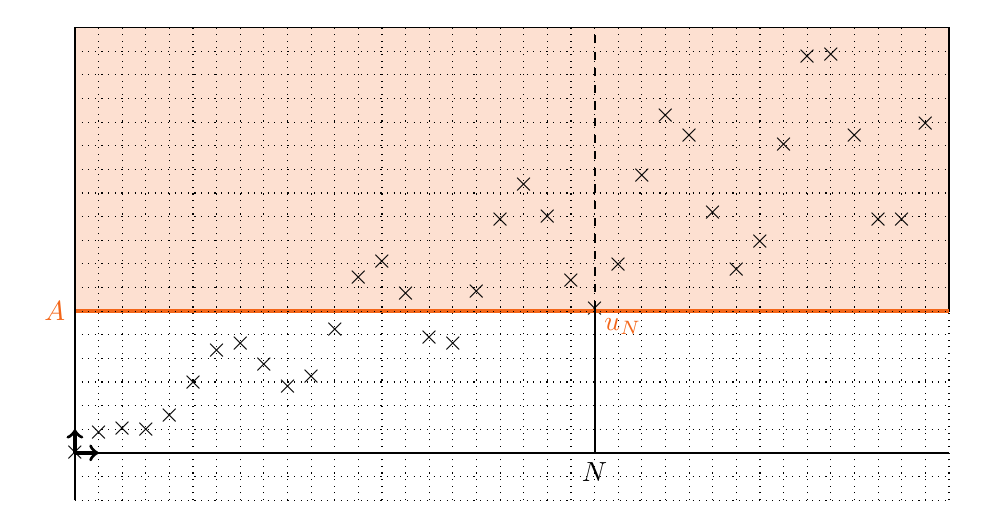
\begin{tikzpicture}[scale=0.3]
\clip (-2,-2) rectangle (38,18);
\draw [fill=ocre!20] (0,6) -- (37,6) -- (37,18) -- (0,18) -- cycle;
\foreach \k in {0,1,...,36} {\draw (\k,{\k^(6/8)*(1.5+cos(deg(\k)))/3+\k/5}) node {$\times$};}

\draw [very thick, ocre, domain = 0:37] plot (\x,6);
\draw [thick] (22,{22^(6/8)*(1.5+cos(deg(22)))/3+22/5}) -- (22,0);
\draw [thick, dashed] (22,{22^(6/8)*(1.5+cos(deg(22)))/3+22/5}) -- (22,18);
\draw [ocre] (22,{22^(6/8)*(1.5+cos(deg(22)))/3+22/5}) node[below right] {$u_{N}$};
\draw  [ocre](0,6) node[left] {$A$};
\draw  (22,0) node[below] {$N$};
\draw [ thin, dotted] (0,-2) grid (37,28);
\draw [thick] (0,0)--(37,0);
\draw [thick] (0,-2)--(0,28);
\draw [->, very thick] (0,0)--(1,0);
\draw [->,very thick] (0,0)--(0,1);

\end{tikzpicture}

\end{center}

On remarque que $u_{12} \geqslant 6$. Cependant, certains des termes suivants sont inférieurs à 6 : pour qu'une suite tende vers $+\infty$, il faut que \textbf{tous les termes} à partir d'un certain rang soient au-dessus du seuil $A$, et ce, peu importe le seuil $A$.
On voit ainsi que, pour tout $n\geqslant 22$, il semblerait qu'on ait bien $u_n \geqslant 6$.

Le raisonnement que nous venons de tenir pour $A=6$ tient pour toutes les valeurs de $A$, aussi grandes soient-elles : la suite $(u_n)$ tend vers $+\infty$.

Naturellement, plus la valeur de $A$ est grande, plus la valeur à partir de laquelle tous les termes de la suite sont tous plus grands que $A$ sera lointaine.

Il faut par ailleurs remarquer et insister \textbf{lourdement} sur le fait qu'une suite qui tend vers $+\infty$ n'est pas forcément croissante. Cette suite ici représentée en est un exemple. Il est également faux de dire qu'une suite qui est strictement croissante tend forcément vers $+\infty$.

\newpage

\begin{example} Pour tout $n$, on pose $u_n=n^2$. $u_n$ tend vers $+\infty$ lorsque $n$ tend vers $+\infty$. 

En effet, fixons un réel $A$.
\begin{itemize}
\item Si $A<0$, alors pour tout entier naturel $n$, on aura $u_n > A$.
\item Si $A \geqslant 0$, alors pour tout entier $n$ supérieur ou égal à $\sqrt{A}$, on a $n^2 \geqslant \sqrt{A}^2$, par croissance de la fonction $x \mapsto x^2$ sur $\mathbb{R}+$. Ceci revient à dire que $u_n \geqslant A$.
\end{itemize}
Dans tous les cas, à partir d'un certain rang, tous les termes de la suite $(u_n)$ sont au-dessus de $A$, peu importe le réel $A$ choisi : la suite $(u_n)$ tend donc vers $+\infty $.
\end{example}

Il y a une différence entre une suite qui tend vers $+\infty$ et une suite non majorée. : évidemment, toute suite qui tend vers $+\infty$ n'est pas majorée, puisque pour tout réel $A$, il y a des termes de la suite supérieurs à $A$.

La réciproque est en revanche fausse sans davantage d'hypothèse sur la suite. Considérons par exemple la suite $(u_n)$ définie pour tout entier naturel $n$ par $u_n=(1+(-1)^n) \, n$. La suite $(u_n)$ n'est pas majorée : elle a des termes arbitrairement grands. Cependant, elle ne tend pas non plus vers $+\infty$ puisqu'un terme sur deux de cette suite vaut 0. Elle ne reste donc pas supérieure à n'importe quel réel donné à partir d'un certain rang (elle est en particulier en dessous de 1 tous les termes impairs).

\subsection{Limite finie : suite convergente}

\begin{definition}Soit $(u_n)$ une suite réelle et $\ell$ un réel. 

On dit que $u_n$ tend vers $\ell$ lorsque $n$ tend vers $+\infty$ si, pour tout $\varepsilon >0$, l'intervalle $] \ell- \varepsilon, \ell+\varepsilon [$ contient tous les termes de la suite $(u_n)$ à partir d'un certain rang.

Autrement dit, pour tout $\varepsilon >0$, il existe un entier $N$ tel que, dès que $n\geqslant N$, on a $|u_n- \ell | \leqslant \varepsilon$.\end{definition}

\textbf{Illustration :} On a représenté graphiquement une certaine suite $(u_n)$ ci-dessous. \begin{center}

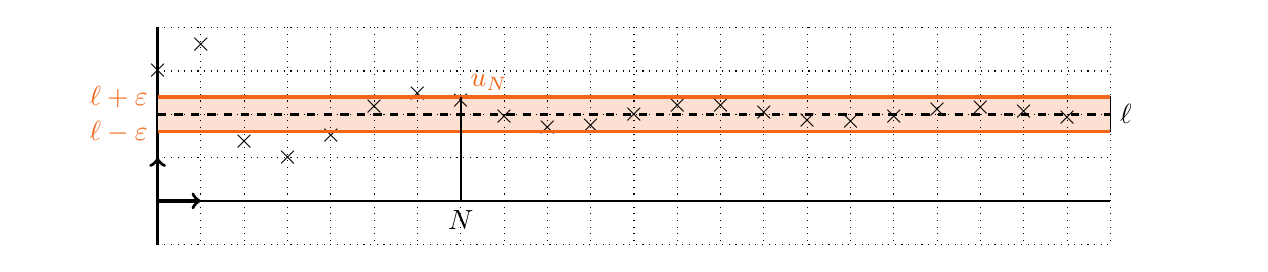
\begin{tikzpicture}[scale=0.55]
\clip (-3,-1) rectangle (25,4);
\draw [thick] (0,0)--(22,0);
\draw [thick] (0,-2)--(0,28);
\draw [->, very thick] (0,0)--(1,0);
\draw [->,very thick] (0,0)--(0,1);

\draw [fill=ocre!20] (0,1.6) -- (22,1.6) -- (22,2.4) -- (0,2.4) -- cycle;
\foreach \k in {1,2,...,21} {\draw (\k,{2+3*cos(deg(\k))/\k}) node {$\times$};}
\draw (0,3) node {$\times$};
\draw [ thin, dotted] (0,-2) grid (22,28);
\draw [very thick, ocre, domain = 0:22] plot (\x,1.6);
\draw [very thick, ocre, domain = 0:22] plot (\x,2.4);
\draw [very thick, dashed, domain = 0:22] plot (\x,2);

\draw [thick] (7,{2+3*cos(deg(7))/7}) -- (7,0);
\draw [thick, dashed] (7,{2+3*cos(deg(7))/7}) -- (7,2.4);
\draw [ocre] (7,{2+3*cos(deg(7))/7}) node[above right] {$u_{N}$};
\draw  [ocre](0,1.6) node[left] {$\ell-\varepsilon$};
\draw  [ocre](0,2.4) node[ left] {$\ell+\varepsilon$};
\draw  (22,2) node[right] {$\ell$};
\draw  (7,0) node[below] {$N$};



\end{tikzpicture}
\end{center}

La suite $(u_n)$ semble tendre vers 2. Par exemple, pour $\varepsilon = 0,4$, tous les termes de la suite sont dans l'intervalle $]2-\varepsilon ; 2+\varepsilon[$, soit $]1,6\,;\, 2,4[$ à partir du rang 7. Ce raisonnement vaut pour n'importe quel $\varepsilon$, aussi petit soit-il.


\begin{proposition}
Soit $(u_n)$ une suite réelle, $\ell$ et $\ell'$ deux réels. Si $u_n$ tend vers $\ell$ et $u_n$ tend vers $\ell'$ lorsque $n$ tend vers $+\infty$, alors $\ell=\ell'$.\end{proposition}

L'idée de la démonstration suivante est assez simple : elle consiste à montrer l'impossibilité d'être à la fois très proche de $\ell$ et de $\ell'$ si ces deux valeurs sont différentes. Pour cela, on va trouver une valeur de $\varepsilon$ pour lesquels les intervalles $] \ell- \varepsilon, \ell+\varepsilon [$ et $] \ell'- \varepsilon, \ell'+\varepsilon [$ sont disjoints, ce qui contredira le fait que ces deux intervalles doivent tous deux contenir tous les termes de la suite à partir d'un certain rang.

\begin{center}
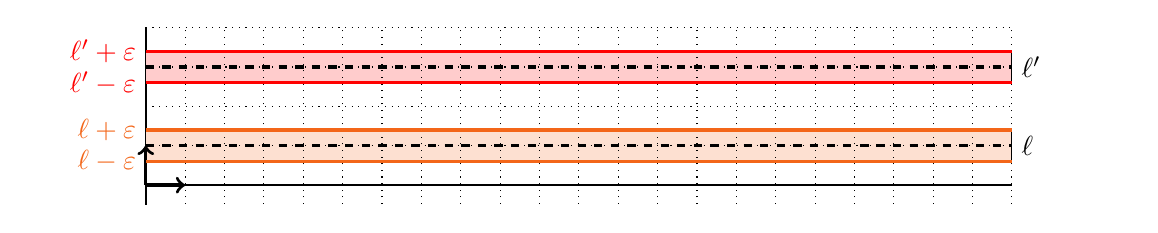
\begin{tikzpicture}[scale=0.5]
\clip (-3,-0.5) rectangle (25,4);
\draw [thick] (0,0)--(22,0);
\draw [thick] (0,-2)--(0,28);


\draw [fill=ocre!20] (0,0.6) -- (22,0.6) -- (22,1.4) -- (0,1.4) -- cycle;
\draw [fill=red!20] (0,2.6) -- (22,2.6) -- (22,3.4) -- (0,3.4) -- cycle;
\draw [->, very thick] (0,0)--(1,0);
\draw [->,very thick] (0,0)--(0,1);

\draw [ thin, dotted] (0,-2) grid (22,28);

\draw [very thick, ocre, domain = 0:22] plot (\x,0.6);
\draw [very thick, ocre, domain = 0:22] plot (\x,1.4);
\draw [very thick, dashed, domain = 0:22] plot (\x,1);

\draw  [ocre](0,0.6) node[left] {$\ell-\varepsilon$};
\draw  [ocre](0,1.4) node[ left] {$\ell+\varepsilon$};
\draw  (22,1) node[right] {$\ell$};


\draw [very thick, red, domain = 0:22] plot (\x,2.6);
\draw [very thick, red, domain = 0:22] plot (\x,3.4);
\draw [very thick, dashed, domain = 0:22] plot (\x,3);

\draw  [red](0,2.6) node[left] {$\ell'-\varepsilon$};
\draw  [red](0,3.4) node[ left] {$\ell'+\varepsilon$};
\draw  (22,3) node[right] {$\ell'$};
\end{tikzpicture}
\end{center}

\begin{demonstration}Supposons que $\ell \neq \ell'$, par exemple que $\ell>\ell'$. Soit $\varepsilon$ un réel strictement positif.
\begin{itemize}
\item Puisque $u_n$ tend vers $\ell$ en $+\infty$, l'intervalle $] \ell- \varepsilon, \ell+\varepsilon [$ contient tous les termes de la suite à partir d'un certain rang $N$. En particulier, à partir d'un certain rang $N$, tous les termes de la suite sont strictement supérieurs à $\ell-\varepsilon $ \item Puisque $u_n$ tend vers $\ell'$ en $+\infty$, l'intervalle $] \ell'- \varepsilon, \ell'+\varepsilon [$ contient tous les termes de la suite à partir d'un certain rang. En particulier, à partir d'un certain rang $N'$, tous les termes de la suite sont strictement inférieurs à $\ell'+\varepsilon $
\end{itemize}
Ainsi, à partir de la plus grande valeur entre $N$ et $N'$, les termes de la suite sont à la fois strictement supérieurs à $\ell-\varepsilon$ et strictement inférieurs à $\ell'+\varepsilon$. Autrement dit, pour tout entier $n \geqslant \max(N,N')$, on a $ \ell-\varepsilon < u_n < \ell'+\varepsilon$.

 Puisque cela vaut pour n'importe quelle valeur de $\varepsilon$, cela reste vrai en prenant par exemple $\varepsilon = \dfrac{\ell-\ell'}{2}$ (ce réel est bien strictement positif puisque $\ell>\ell'$).

Ainsi, pour tout entier $n\geqslant \max(N,N')$, on a $\ell-\dfrac{\ell-\ell'}{2}< u_n < \ell'+\dfrac{\ell-\ell'}{2}$ et donc $\dfrac{\ell+\ell'}{2} < u_n < \dfrac{\ell+\ell'}{2}$ et en particulier $\dfrac{\ell+\ell'}{2} < \dfrac{\ell+\ell'}{2}$. C'est impossible : notre supposition de départ, qui était que $\ell \neq \ell'$ était donc erroné. Par conséquent, on a $\ell=\ell'$.

Le raisonnement que nous venons d'appliquer, qui consiste, en supposant une proposition vraie, à aboutir à une conclusion fausse et à en déduire que la proposition de départ devait donc également être fausse s'appelle le \textbf{raisonnement par l'absurde}.\end{demonstration}


Cette propriété nous permet de définir sans ambiguïté la notion de limite d'une suite.

\begin{definition}[Limite finie, suite convergente] Soit $(u_n)$ une suite réelle et $\ell$ un réel. 

Si $u_n$ tend vers $\ell$ lorsque $n$ tend vers $+\infty$, on dit que $\ell$ est \textbf{LA} \textit{limite} de la suite $(u_n)$ lorsque $n$ tend vers $+\infty$. On note alors $\displaystyle \lim _{ n \to +\infty} u_n = \ell$.


Une suite qui admet une limite finie est dite \textit{convergente}. 

Dans le cas contraire, on parle de suite \textit{divergente} : cela regroupe les suites qui ont une limite infinie mais aussi les suites qui n'admettent pas de limite.\end{definition}



\begin{example} Pour tout entier naturel $n$, on pose $u_n=\dfrac{2n+1}{4n+5}$. \\
Pour se faire une idée de la limite, il est possible de calculer quelques termes de la suite. Ainsi, $u_0=\dfrac{1}{5}$, $u_{10}=\dfrac{21}{45}\simeq 0.467$, $u_{100} = \dfrac{201}{405} \simeq 0.496$... Il semble que la suite soit convergente et que sa limite vaille $\dfrac{1}{2}$.
\vskip15pt
Pour le prouver formellement, repassons pas la définition  : pour n'importe quel $\varepsilon >0$, il faut trouver un rang $N$ à partir duquel, pour tout $n>N$, on ait $u_n \in \left] \dfrac{1}{2}-\varepsilon ; \dfrac{1}{2}+\varepsilon \right[$.

Soit $n\in\mathbb{N}$, 
\[u_n-\dfrac{1}{2}=\dfrac{2n+1}{4n+5}-\dfrac{1}{2}=\dfrac{4n+2}{2(4n+5)}-\dfrac{4n+5}{2(4n+5)}=\dfrac{-3}{2(4n+5)}\]
Cette quantité est négative. On a alors \[\left\lvert u_n - \dfrac{1}{2} \right\rvert = \dfrac{3}{2(4n+5)}\]

Fixons alors $\varepsilon >0$. Ainsi, 
\[ \left\lvert u_n - \dfrac{1}{2} \right\rvert < \varepsilon \Leftrightarrow \dfrac{3}{2(4n+5)} < \varepsilon \Leftrightarrow \dfrac{1}{4n+5}<\dfrac{2\varepsilon}{3} \Leftrightarrow 4n+5 > \dfrac{3}{2\varepsilon} \Leftrightarrow n > \dfrac{3}{8\varepsilon}-\dfrac{5}{4} \]
Ainsi, pour tout $\varepsilon >0$, dès que $n  > \dfrac{3}{8\varepsilon}-\dfrac{5}{4}$, on a $u_n \in \left] \dfrac{1}{2}-\varepsilon ; \dfrac{1}{2}+\varepsilon \right[$. La suite $(u_n)$ est bien convergente et sa limite vaut $\dfrac{1}{2}$.

Par exemple, si $\varepsilon = 0.001$, on a $\dfrac{3}{8\varepsilon}-\dfrac{5}{4}= 374.99$. 

Ainsi, pour tout entier $n\geqslant 375$, on a  $0.499 \leqslant u_n \leqslant 0.501$.\end{example}

Nous verrons très bientôt des résultats qui nous permettront de passer outre cet aspect formel. Même si une telle démonstration de la convergence d'une suite n'est que rarement demandée en classe de terminale, comprendre les bases de ce raisonnement constituera un avantage certain dans les études supérieures.

\begin{proposition}Si une suite est convergente, elle est bornée. Par contraposée, si une suite n'est pas bornée, elle ne peut être convergente.\end{proposition}

 La réciproque est fausse : toute suite bornée n'est pas convergente. 
 
Par exemple, pour tout $n$, prenons $u_n=(-1)^n$. La suite $(u_n)$ est bornée puisque, pour tout $n$, $-1 \leqslant u_n \leqslant 1$. En revanche, elle n'est pas convergente : ses termes de rangs pairs valent tous $1$ et ses termes de rangs impairs valent tous $-1$. Une limite étant unique, la suite $(u_n)$ ne peut être convergente.

\subsection{Limites de suites usuelles}

\begin{proposition} Les limites suivantes sont à connaître.
\begin{center}
\begin{tabularx}{0.9\linewidth}{XXX}
 $\displaystyle \lim _{n\to+\infty} n = + \infty$ & $\displaystyle \lim _{n\to+\infty} n^{2} = + \infty$ &  $\displaystyle \lim _{n\to+\infty} \dfrac{1}{n} = 0$ \end{tabularx}
\end{center}

Plus généralement, pour tout entier naturel non nul $\alpha$, $\displaystyle \lim _{n\to+\infty} n^{\alpha} = + \infty$ et $\displaystyle \lim _{n\to+\infty} \dfrac{1}{n^{\alpha}} = 0$.
\begin{center}
\begin{tabularx}{0.9\linewidth}{XXX}
  $\displaystyle \lim _{n\to+\infty} \sqrt{n} = + \infty$ & $\displaystyle \lim _{n\to+\infty} \e^n = + \infty$ & $\displaystyle \lim _{n\to+\infty} \e^{-n} = 0$\end{tabularx}
\end{center}

 Les suites $(\cos(n))$, $(\sin(n))$ et $((-1)^n)$ n'admettent quant à elles pas de limite lorsque $n$ tend vers $+\infty$.
\end{proposition}

\newpage
\section{Opérations sur les limites}

\subsection{Limite de la somme}

\begin{proposition}On considère deux suites réelles $(u_n)$ et $(v_n)$ et deux réels $\ell_1$ et $\ell_2$. 

\begin{tabularx}{\linewidth}{|l|X|X|X|X|X|X|}
\hline
$\displaystyle \lim_{n \to +\infty} u_n$ & $\ell_1$ & $\ell_1$ & $\ell_1$ & $+\infty$ & $-\infty$ & $+\infty$\\
\hline
$\displaystyle \lim_{n \to +\infty} v_n$ & $\ell_2$ & $+\infty$ & $-\infty$ & $+\infty$ & $-\infty$ & $-\infty$\\
\hline
$\displaystyle \lim_{n \to +\infty} (u_n + v_n)$ & $\ell_1+\ell_2$ & $+\infty$ & $-\infty$ & $+\infty$ & $-\infty$ & \textbf{Indéterminé} \\
\hline
\end{tabularx}\end{proposition}

\begin{demonstration}Bien qu'elles ne soient pas explicitement au programme, les démonstrations de ces résultats permettent de manipuler et comprendre les définitions des différentes limites de suite. 

On s'intéresse ici au cas où $\displaystyle\lim_{n \to + \infty}u_n=+\infty$ et $\displaystyle \lim_{n \to+\infty}v_n=+\infty$. Les autres démonstrations pourront être traitées en guise d'exercice.

Soit donc $A$ un réel.
\begin{itemize}
\item Puisque $\displaystyle\lim_{n \to + \infty}u_n=+\infty$, il existe un entier naturel $N_1$ tel que, pour tout entier $n\geqslant N_1$, on a $u_n \geqslant A$.
\item Puisque $\displaystyle\lim_{n \to + \infty}v_n=+\infty$, il existe un entier naturel $N_2$ tel que, pour tout entier $n\geqslant N_2$, on a $u_n \geqslant 0$.
\end{itemize}
Posons alors $N=\max (N_1,N_2)$. Alors, pour tout entier naturel $n \geqslant N$, on a $u_n + v_n \geqslant A + 0$ et donc $u_n+v_n\geqslant A$. Ainsi, on a montré que $\displaystyle \lim_{n \to+\infty}(u_n+v_n)=+\infty$\end{demonstration}

\begin{example}Pour tout entier naturel $n$, on pose $u_n=n^2+\e^{-n}-4$. 

On sait que $\displaystyle \lim_{n \to +\infty} n^2 = +\infty$,  $\displaystyle \lim_{n \to +\infty} \e^{-n} = 0$ et $\displaystyle \lim_{n \to +\infty} (-4)= -4$. Ainsi, $\displaystyle \lim_{n \to +\infty} u_n =+\infty$.\end{example}

Les cas où $\displaystyle \lim_{n \to +\infty} u_n = +\infty$ et $\displaystyle \lim_{n \to +\infty} v_n = -\infty$ n'obéissent à aucune règle précise : il faut les traiter séparément. L'expression "Forme indéterminée" ne signifie pas qu'il est impossible de déterminer une éventuelle limite : il précise simplement qu'il nous est impossible d'appliquer directement les règles de calcul sur les limites de suite. 

La limite de la somme peut alors aussi bien être 0, 1, $+\infty$, $-\infty$ ou peut même ne pas exister du tout !

\begin{example} Pour tout entier naturel $n$, on pose $u_n = n$, $v_n = 1-n$ et $w_n=n^2+n$.

On a alors $\displaystyle \lim_{n \to +\infty} u_n = +\infty$ et $\displaystyle \lim_{n \to +\infty} v_n = -\infty$. Il n'est pas possible de conclure sur l'éventuelle limite de la suite $(u_n+v_n)$ avec ces seules informations.

Or, pour tout entier naturel $n$, $u_n+v_n=1$ et on en déduit que $\displaystyle \lim_{n \to +\infty} (u_n+v_n) = 1$.

Par ailleurs, $\displaystyle \lim_{n \to +\infty} w_n = +\infty$ et $\displaystyle \lim_{n \to +\infty} v_n = -\infty$. Là encore, il n'est pas possible de conclure sur l'éventuelle limite de la suite $(v_n+w_n)$ avec ces seules informations.

Or, pour tout entier naturel $n$, $v_n+w_n=n^2+1$. Ainsi, $\displaystyle \lim_{n \to +\infty} (v_n+w_n) = +\infty$. 

Nous avons là deux exemples où la somme de limites "$\infty - \infty $" produit des résultats totalement différents.\end{example}

\newpage

\subsection{Limite du produit}



\begin{proposition}On considère deux suites réelles $(u_n)$ et $(v_n)$ et deux réels $\ell_1$ et $\ell_2$. 
\vskip10pt
\begin{tabularx}{\linewidth}{|l|X|X|X|X|}
\hline
$\displaystyle \lim_{n \to +\infty} u_n$ & $\ell_1 $ & $\ell_1 \neq 0$ &  $\infty$ & $0$ \\
\hline
$\displaystyle \lim_{n \to +\infty} v_n$ & $\ell_2$ & $\infty$  & $\infty$  & $\infty$ \\
\hline
$\displaystyle \lim_{n \to +\infty} (u_n \, v_n)$ & $\ell_1\,\ell_2$ & $\infty$ (r.s.)  & $\infty$ (r.s.) & \textbf{Indéterminé} \\
\hline
\end{tabularx}

\begin{center}
 \textbf{r.s. : Règle des signes}
 \end{center} \vspace{-1cm} \end{proposition}

\begin{example} Pour tout entier naturel non nul $n$, on pose $u_n = \left(\dfrac{3}{n}-4\right)\times (n^2+2\sqrt{n})$.
\begin{itemize}
\item $\displaystyle \lim_{n \to +\infty} \dfrac{3}{n} = 0$ donc $\displaystyle \lim_{n \to +\infty} \left( \dfrac{3}{n}-4 \right) = -4$.
\vskip5pt
\item $\displaystyle \lim_{n \to +\infty} n^2 = +\infty$ et $\displaystyle \lim_{n \to +\infty} \sqrt{n} = +\infty$. Ainsi, $\displaystyle \lim_{n \to +\infty} (n^2+ \sqrt{n})=+\infty$.
\vskip5pt
\item Finalement, d'après les règles de calcul de limite d'un produit, $\displaystyle \lim_{n \to +\infty} u_n = -\infty$.\end{itemize}
\end{example}

\begin{example} Pour tout entier naturel non nul $n$, on pose $u_n=\dfrac{2}{n}$, $v_n=n$ et $w_n=n^2$. 
\begin{itemize}
\item On a $\displaystyle \lim_{n \to +\infty} u_n = 0$, $\displaystyle \lim_{n \to +\infty} v_n = + \infty$. Par ailleurs, pour tout entier naturel non nul $n$, $u_n \, v_n = 2$. Ainsi, $\displaystyle \lim_{n \to +\infty} (u_n \, v_n) = 2$.
\vskip5pt
\item On a $\displaystyle \lim_{n \to +\infty} u_n = 0$, $\displaystyle \lim_{n \to +\infty} w_n = + \infty$. Par ailleurs, pour tout entier naturel non nul $n$, $u_n \, w_n = 2n$. Ainsi, $\displaystyle \lim_{n \to +\infty} (u_n \, v_n) = +\infty$.
\end{itemize} 
On voit sur cet exemple que le produit d'une limite infinie et d'une limite qui vaut 0 peut aboutir à plusieurs résultats différents.\end{example}



\subsection{Limite du quotient}


\begin{definition}Soit $(u_n)$ une suite réelle et $a$ un réel. 

\begin{itemize}
\item On note $\displaystyle\lim_{n \to +\infty}u_n = a^+$ si $u_n$ tend vers $a$ lorsque $n$ tend vers $+\infty$ ET s'il existe un entier $N$ tel que, pour tout entier naturel $n$ supérieur à $N$, on a $u_n \geqslant a$.
\item On note $\displaystyle\lim_{n \to +\infty}u_n = a^-$ si $u_n$ tend vers $a$ lorsque $n$ tend vers $+\infty$ ET s'il existe un entier $N$ tel que, pour tout entier naturel $n$ supérieur à $N$, on a $u_n \leqslant a$.\end{itemize}
\end{definition}

\begin{example}On sait que $\displaystyle\lim_{n \to + \infty}\left(1-\dfrac{1}{n}\right)=1$. Or, pour tout entier naturel non nul $n$, $1-\dfrac{1}{n}\leqslant 1$. On pourra alors écrire $\displaystyle\lim_{n \to + \infty}\left(1-\dfrac{1}{n}\right)=1^-$.\end{example}

Cette petite subtilité nous est notamment utile lorsque l'on étudie la limite de quotients dans certains cas...


\begin{proposition}On considère deux suites réelles $(u_n)$ et $(v_n)$ telles que $(v_n)$ ne s'annule pas à partir d'un certain rang. On considère deux réels $l_1$ et $l_2$, avec $l_2 \neq 0$. 
\vskip10pt
\begin{tabularx}{\linewidth}{|l|X|X|X|X|c|c|}
\hline
$\displaystyle \lim_{n \to +\infty} u_n$ & $\ell_1 $ & $\ell_1$ & $\ell_1 \neq 0$ & $\infty$  & $0$ & $\infty$\\
\hline
$\displaystyle \lim_{n \to +\infty} v_n$ & $\ell_2 \neq 0$ & $\infty$ &  $0^+$ ou $0^-$ &  $l_2$, $0^+$ ou $0^-$ & $0$ & $\infty$ \\
\hline
$\displaystyle \lim_{n \to +\infty} \left(\dfrac{u_n}{ v_n}\right)$ & $\dfrac{\ell_1}{\ell_2}$ & 0 & $\infty$  (r.s.)  & $\infty$ (r.s.) & \multicolumn{2}{|c|}{\textbf{Indéterminé}} \\
\hline\end{tabularx}


\begin{center}
 \textbf{r.s. : Règle des signes}\\
 \end{center} 
 \vspace{-1cm}\end{proposition}
 
\begin{example} Pour tout entier naturel non nul $n$ on pose $u_n=\dfrac{1+\frac{2}{n}}{3+n}$.

On a  $\displaystyle \lim_{n \to +\infty} \left(1+\dfrac{2}{n}\right)=1$ et $\displaystyle \lim_{n \to +\infty} (3+n) = +\infty$. Ainsi, $\displaystyle \lim_{n \to +\infty} u_n = 0$.\end{example}


\begin{example} Pour tout entier naturel non nul $n$ on pose $u_n=\dfrac{1-n}{\e^{-n}+\frac{1}{n}}$.

On a  $\displaystyle \lim_{n \to +\infty} \left(1-n\right)=-\infty$ et $\displaystyle \lim_{n \to +\infty}\left(\e^{-n}+\frac{1}{n}\right) = 0$. Par ailleurs, pour tout entier naturel non nul $n$, $\e^{-n}+\frac{1}{n} \geqslant 0$. On a en fait $\displaystyle \lim_{n \to +\infty}\left(\e^{-n}+\frac{1}{n}\right) = 0^+$

Ainsi, $\displaystyle \lim_{n \to +\infty} u_n = -\infty$ (ne pas oublier d'appliquer la règle des signes !).\end{example}




\section{Formes indéterminées}

\subsection{Factorisation par le terme dominant}

\begin{example} Pour tout entier naturel $n$, on pose $u_n=4n^2+2n+3$ et $v_n = 3n^2+7n-1$. 

On cherche à déterminer $\displaystyle \lim_{n \to +\infty} \dfrac{u_n}{v_n}$. Or, en utilisant les règles sur les calculs de limites, on trouve que $\displaystyle \lim_{n \to +\infty} u_n = +\infty$ et $\displaystyle \lim_{n \to +\infty} v_n = +\infty$. On se retrouve dans le cas "$\dfrac{\infty}{\infty}$".

Il est toutefois possible de factoriser $u_n$ et $v_n$ par leur terme de plus haut degré (ici, $n^2$ dans les deux cas). Pour tout entier non nul $n$, on a donc 
\[ \dfrac{u_n}{v_n}=\dfrac{4n^2+2n+3}{3n^2+7n-1}=\dfrac{n^2\left(4+\dfrac{2}{n}+\dfrac{3}{n^2}\right)}{n^2\left(3+\dfrac{7}{n}-\dfrac{1}{n^2}\right)}=\dfrac{4+\dfrac{2}{n}+\dfrac{3}{n^2}}{3+\dfrac{7}{n}-\dfrac{1}{n^2}}.\]

Or,  $\displaystyle \lim_{n \to +\infty}\left(4+\dfrac{2}{n}+\dfrac{3}{n^2}\right) = 4$ et $\displaystyle \lim_{n \to +\infty} \left(3+\dfrac{7}{n}-\dfrac{1}{n^2}\right) = 3$.

Ainsi, $\displaystyle \lim_{n \to +\infty} \dfrac{u_n}{v_n} = \dfrac{4}{3}$.
\end{example}

Il est à noter qu'avant de se lancer dans la factorisation par le terme dominant, il faut s'assurer que celle-ci est nécessaire : en voulant lever une forme indéterminée inexistante, on peut très vite se retrouver à en créer une involontairement.

\subsection{Quantité conjuguée}

La partie suivante s'intéresse aux formes indéterminées faisant intervenir des racines carrées.

\begin{proposition}Soit $(u_n)$ une suite réelle positive et $a$ un réel positif.
\begin{itemize}
\item Si $\displaystyle \lim_{n \to +\infty} u_n=a$, alors $\displaystyle \lim_{n \to +\infty} \sqrt{u_n}=\sqrt{a}$.
\item Si $\displaystyle \lim_{n \to +\infty} u_n=+\infty$, alors $\displaystyle \lim_{n \to +\infty} \sqrt{u_n}=+\infty$.
\end{itemize}\end{proposition}

\begin{example}Pour tout entier naturel non nul $n$, on pose $u_n = \dfrac{\sqrt{4n^2+1}}{n}$.

D'une part, pour tout entier naturel non nul $n$, $4n^2+1=n^2\left(4+\dfrac{1}{n^2}\right)$ et donc 
\[\sqrt{4n^2+1}=\sqrt{n^2\left(4+\dfrac{1}{n^2}\right)}=\sqrt{n^2}\times \sqrt{4+\dfrac{1}{n^2}}=n \times  \sqrt{4+\dfrac{1}{n^2}}.\]
Ainsi, pour tout entier naturel $n$, $u_n=\sqrt{4+\dfrac{1}{n^2}}$. Or, $\displaystyle\lim_{n\to + \infty}\left(4+\dfrac{1}{n^2}\right)=4$ et donc $\displaystyle\lim_{n\to + \infty} u_n = \sqrt{4}=2$.\end{example}

Lorsque l'on est en présence d'une différence de racines carrées $\sqrt{a}-\sqrt{b}$, on peut multiplier et diviser par la quantité conjuguée $\sqrt{a}+\sqrt{b}$.

L'objectif est ici d'utiliser l'identité remarquable $(x-y)(x+y)=x^2-y^2$. En particulier, dans le cas des racines carrées, cela entraîne que, pour tous réels strictement positifs $a$ et $b$,\[(\sqrt{a}-\sqrt{b})(\sqrt{a}+\sqrt{b})=\sqrt{a}^2-\sqrt{b}^2=a-b.\]

\begin{example} Pour tout entier naturel non nul $n$, on note $u_n=\sqrt{n+1}-\sqrt{n-1}$. Il s'agit de la différence de deux termes qui tendent vers $+\infty$, il n'est pas possible de conclure directement sur sa limite. Or,
\[ u_n = (\sqrt{n+1}-\sqrt{n-1}) \times \dfrac{\sqrt{n+1}+\sqrt{n-1}}{\sqrt{n+1}+\sqrt{n-1}}=\dfrac{n+1-(n-1)}{\sqrt{n+1}+\sqrt{n-1}}=\dfrac{2}{\sqrt{n+1}+\sqrt{n-1}}.\]
Le numérateur vaut 2 et le dénominateur tend vers $+\infty$. Ainsi, $\displaystyle \lim_{n \to +\infty} u_n = 0$.
\end{example}

\newpage


\chapter{Exercices}
\setcounter{section}{0}

\section*{Limite d'une suite}

\begin{exercise} Pour tout entier naturel $n$, on pose $u_n=\sqrt{n}$.
\begin{enumerate}
\item Résoudre l'inéquation $u_n \geqslant 100$.
\item Résoudre l'inéquation $u_n \geqslant 100000$.
\item Soi $A$ un réel quelconque. Résoudre l'inéquation $u_n \geqslant A$.
\item Que peut-on en déduire sur la limite de la suite $(u_n)$ ?
\end{enumerate}
\end{exercise}
\begin{solution}Puisque $n \geqslant 0$, $u_n \geqslant 100$ si et seulement si $n \geqslant 100^2$ c'est-à-dire $n \geqslant 10000$.

Puisque $n \geqslant 0$, $u_n \geqslant 100000$ si et seulement si $n \geqslant 100^2$ c'est-à-dire $n \geqslant 10000000000$.

On considère un réel $A$ quelconque.
\begin{itemize}
\item Si $A<0$, alors pour tout $n$, $u_n>A$.
\item Si $A\geqslant 0$, on sait que $\sqrt{n} \geqslant A \Leftrightarrow n \geqslant A^2$. Ainsi, dès que $n\geqslant A^2$, on a $u_n \geqslant A$ et ceci est valable quelque soit la valeur de $A$.
\end{itemize}

Puisque pour tout $A$, on a $u_n \geqslant A$ à partir d'un certain rang, on peut en conclure que $\displaystyle \lim _{n\to +\infty} u_n = +\infty$.\end{solution}



\begin{exercise}On considère la suite $(u_n)$ définie pour tout $n\in \mathbb{N}$ par  $u_n=4-3n$.
\begin{enumerate}
\item Calculer $u_{30}$, $u_{70}$, $u_{1000}$. Quelle semble être la limite de la suite $(u_n)$ ?
\item Soit $A$ un réel. Résoudre l'équation $u_n \leqslant A$, d'inconnue $n\in\mathbb{N}$.
\item Que peut-on en conclure sur la limite de la suite $(u_n)$ ?
\end{enumerate}
\end{exercise}
\begin{solution}On a $u_{30}=-86$, $u_{70}=-206$, $u_{1000}=-2996$. Il semble que la limite de la suite $(u_n)$ soit $-\infty$.

$u_n\leqslant A$ si et seulement si $4-3n \leqslant A$ si et seulement si $n\geqslant \dfrac{A-4}{-3}$. Puisque pour tout réel $A$, on a $u_n \leqslant A$ à partir d'un certain rang, on peut en conclure que $\displaystyle \lim _{n\to +\infty} u_n = -\infty$.\end{solution}




\begin{exercise}Pour tout $n\in\mathbb{N}$, on note $u_n=\left\{\begin{array}{ll} 1 & \text{si } n \text{ est premier}\\
n^2 & \text{sinon}

\end{array}\right.$. A-t-on $\displaystyle \lim _{n\to +\infty} u_n = +\infty$ ?\end{exercise}
\begin{solution}Cette suite tend pas vers $+\infty$. En effet, on rappelle qu'il existe une infinité de nombres premiers, et donc une infinité de valeur de $n$ pour lesquels $u_n = 1$. Prenons en particulier $A=2$ dans la définition de la limite infinie. On a donc que, pour tout $N$, il existe un rang $n \geqslant N$ tel que $u_n < 2$ : il n'est pas possible d'avoir tous les termes de la suite supérieurs à 2 à partir d'un certain rang. La limite de la suite ne peut donc être $+\infty$. \end{solution}




\begin{exercise}Pour tout $n\in\mathbb{N}$, on pose $u_n=\dfrac{3-5n}{10n+2}$. Quelle semble être la limite de la suite $(u_n)$ ?\end{exercise}
\begin{solution}Il semble que la limite de la suite $(u_n)$ soit $-\dfrac{1}{2}$.\end{solution}



\begin{exercise}On considère la suite $(u_n)$ définie par $u_0=12$ et pour tout entier naturel $n$, $u_{n+1}= \dfrac{u_n}{2}+2$. 

\begin{enumerate}
\item Quelle semble être la limite de la suite $(u_n)$ ?
\item Cette limite change-t-elle si $u_0=3$ ?\end{enumerate}\end{exercise}
\begin{solution}Il semblerait que la limite de cette suite soit 4. On obtient la même limite si on prend $u_0=3$.\end{solution}




\begin{exercise}


On considère la suite $(u_n)$ définie pour tout $n\in\mathbb{N}$ par $u_n=\dfrac{3n+6}{n+1}$.
\begin{enumerate}
\item Donner des valeurs approchées au centième de $u_{10}$, $u_{100}$, $u_{1000}$ .
\item La suite $(u_n)$ semble-t-elle convergente ? Quelle serait sa limite ?
\item Montrer que pour $n\in\mathbb{N}$, $u_n-3=\dfrac{3}{n+1}$. Quel est le signe de cette quantité ?
\item En déduire que $|u_n-3|=u_n-3$. On rappelle que la valeur absolue d'un réel $x$ vaut $x$ si ce réel est positif et $-x$ sinon.
\item Soit $\varepsilon >0$. Résoudre l'inéquation $\left\lvert u_n - 3 \right\rvert < \varepsilon$, d'inconnue $n\in\mathbb{N}$. Conclure.
\end{enumerate}\end{exercise}
\begin{solution}On a $u_{10}=\dfrac{36}{11}\simeq 3.272$, $u_{100}=\dfrac{306}{101}\simeq 3.030$, $u_{1000}=\dfrac{3006}{1001}\simeq 3.003$. Il semblerait que la suite $(u_n)$ soit convergente, de limite 3.

Pour $n\in\mathbb{N}$, $u_n-3=\dfrac{3n+6}{3+1}-\dfrac{3(n+1)}{n+1}=\dfrac{3n+6-3n-3}{n+1}=\dfrac{3}{n+1}$. Puisque cette valeur est positive, on a $|u_n-3|=u_n-3=\dfrac{3}{n+1}$.

Soit $\varepsilon >0$. On a $\left\lvert u_n - 3 \right\rvert < \varepsilon \Leftrightarrow \dfrac{3}{n+1}< \varepsilon \Leftrightarrow \dfrac{n+1}{3} > \dfrac{1}{\varepsilon} \Leftrightarrow n > \dfrac{3}{\varepsilon}-1$.

Ainsi, pour tout $\varepsilon > 0$, dès que $n > \dfrac{3}{\varepsilon}-1$, on a $\left\lvert u_n - 3 \right\rvert < \varepsilon$. Ainsi, la suite $(u_n)$ est convergente et $\displaystyle \lim _{n\to + \infty}u_n=3$.\end{solution}



\begin{exercise}Pour tout entier naturel $n$, on pose $u_n=(-1)^n$. La suite $(u_n)$ semble-t-elle avoir une limite ?\end{exercise}
\begin{solution}Les termes de rang pair de cette suite valent 1 alors que les termes de rang impair valent -1. Cette suite n'admet pas de limite.\end{solution}



\section*{Opérations sur les limites}

\begin{exercise}Dans chacun des cas suivants, déterminer la limite, si elle existe, de la suite $(u_n)$  définie pour tout entier naturel non nul $n$.

\renewcommand{\arraystretch}{2.5}
\begin{tabularx}{\linewidth}{XXX}
\textbf{a.}  $u_n= n^2+\sqrt{n}$ & \textbf{b.} $u_n = \dfrac{1}{n}-n^3$ & \textbf{c.} $u_n = \e^{-n}+3n$ \\
\textbf{d.} $u_n = \dfrac{1}{n} + \dfrac{1}{n^2}+n$ & \textbf{e.} $ u_n =-6n^2+1+ \dfrac{1}{n}$ & \textbf{f.} $u_n=\dfrac{1+n}{n}$\\
\textbf{g.} $u_n = (2n+1)\left(\dfrac{1}{	n}+2\right)$ & \textbf{h.} $ u_n = \left(3+\dfrac{2}{n}\right) \left( \dfrac{5}{n^2}-2\right)$ & \textbf{i.} $u_n=\sqrt{n}-n^2\sqrt{n}$\\
\textbf{j.} $ u_n = \dfrac{\e^n}{1+\frac{1}{n}}$ & \textbf{k.} $ u_n = \dfrac{6+\frac{3}{n^2}}{\frac{5}{n}-1}$ &
\textbf{l.} $ u_n = \dfrac{-1+\frac{3}{n}}{\frac{1}{n^2}}$ \\

\textbf{m.} $u_n=n^2-n$ & \textbf{n.} $u_n=\left(1-\dfrac{1}{n}\right)\left(2+\dfrac{3}{n^2}\right)$ & 
\textbf{o.} $u_n=\dfrac{3+\sqrt{n}}{1+\dfrac{2}{n}}$\\
\textbf{p.} $u_n=-2n^2-\dfrac{5}{n+1}$ & \textbf{q.} $u_n=\dfrac{5}{-1-n}$ & \textbf{r.} $u_n = (3n+1)\left(\dfrac{1}{n}-2\right)$
\end{tabularx}
\end{exercise}
\begin{solution}\textbf{a.} On sait que $\displaystyle \lim _{n\to +\infty} n^2 = +\infty$, $\displaystyle \lim _{n\to +\infty} \sqrt{n} = +\infty$.\\ Ainsi, d'après les règles de la limite de la somme, $\displaystyle \lim _{n\to +\infty} n^2+\sqrt{n} = +\infty$.

\textbf{b.} On sait que $\displaystyle \lim _{n\to +\infty} \dfrac{1}{n} = 0$ et $\displaystyle \lim _{n\to +\infty} -n^3 = -\infty$.\\ Ainsi, d'après les règles de la limite de la somme, $\displaystyle \lim _{n\to +\infty} \left( \dfrac{1}{n}-n^3 \right) = -\infty$;

\textbf{c.} On sait que $\displaystyle \lim _{n\to +\infty} \e^{-n} = 0$ et $\displaystyle \lim _{n\to +\infty} (3n)= +\infty$.\\ Ainsi, d'après les règles de la limite de la somme, $\displaystyle \lim _{n\to +\infty} \left(\e^{-n}+3n\right) = +\infty$.

\textbf{d.} On sait que $\displaystyle \lim _{n\to +\infty} \dfrac{1}{n} = 0$, $\displaystyle \lim _{n\to +\infty} \dfrac{1}{n^2} = 0$ et $\displaystyle \lim _{n\to +\infty} n = +\infty$.\\ Ainsi, d'après les règles de la limite de la somme, $\displaystyle \lim _{n\to +\infty} \left( \dfrac{1}{n}+\dfrac{1}{n^2}+n \right) = +\infty$.
 
\textbf{e.} On sait que $\displaystyle \lim _{n\to +\infty}-n^2 = -\infty$, $\displaystyle \lim _{n\to +\infty} \dfrac{1}{n} = 0$ et $\displaystyle \lim _{n\to +\infty} 1 = 1$.\\ Ainsi, d'après les règles de la limite de la somme, $\displaystyle \lim _{n\to +\infty} \left( -6n^2+1+ \dfrac{1}{n} \right) = -\infty$ .

\textbf{f.} Pour tout entier naturel non nul $n$, $\dfrac{n+1}{n}=\dfrac{1}{n}+\dfrac{n}{n}=1+\dfrac{1}{n}$. On sait que $\displaystyle \lim _{n\to +\infty} \dfrac{1}{n} = 0$ et $\displaystyle \lim _{n\to +\infty} 1 = 1$.\\ Ainsi, d'après les règles de la limite de la somme, $\displaystyle \lim _{n\to +\infty} \left( \dfrac{1+n}{n} \right) = 1$.
 
\textbf{g.} D'une part, $\displaystyle \lim _{n\to +\infty} (2n+1) = +\infty$. D'autre part, $\displaystyle \lim _{n\to +\infty} \dfrac{1}{n} = 0$ d'où $\displaystyle \lim _{n\to +\infty} \left(\dfrac{1}{n}+2\right) = 2$.\\ Ainsi, d'après les règles de calcul de la limite d'un produit, $\displaystyle \lim _{n\to +\infty} (2n+1)\left(\dfrac{1}{n}+2\right) = +\infty$.
 
\textbf{h.} On a $\displaystyle \lim _{n\to +\infty} \dfrac{2}{n}=0$, d'où $\displaystyle \lim _{n\to +\infty} \left(3+\dfrac{2}{n}\right)=3$. D'autre part, $\displaystyle \lim _{n\to +\infty} \dfrac{5}{n^2}=0$ d'où $\displaystyle \lim _{n\to +\infty} \left(\dfrac{5}{n^2}-2\right)=-2$. Finalement, par produit de limites, $\displaystyle \lim _{n\to +\infty} \left(3+\dfrac{2}{n}\right)\left(\dfrac{5}{n^2}-2\right)=3\times (-2)=-6$.

\textbf{i.} Si l'on fait la limite de chaque terme de la somme, on aboutit à une forme indéterminée, de type "$\infty - \infty $". Il faut donc factoriser $u_n$. Pour tout entier $n$, $u_n=\sqrt{n}(1-n^2)$. Or, $\displaystyle \lim _{n\to +\infty} \sqrt{n}=+\infty$ et $\displaystyle \lim _{n\to +\infty} (1-n^2)=-\infty$. Ainsi, $\displaystyle \lim _{n\to +\infty} u_n = -\infty$.

\textbf{j.} D'une part, $\displaystyle \lim_{n \to +\infty} \e^n = +\infty$. D'autre part, $\displaystyle \lim_{n \to +\infty} \dfrac{1}{n} = 0$ d'où $\displaystyle \lim_{n \to +\infty} \left(1+\dfrac{1}{n}\right)=1$.\\ Finalement, $\displaystyle \lim_{n \to +\infty} \dfrac{\e^n}{1+\dfrac{1}{n}}=+\infty$.

\textbf{k.} On a, $\displaystyle \lim_{n \to +\infty} \dfrac{3}{n^2}=0$ d'où $\displaystyle \lim_{n \to +\infty} \left(6+\dfrac{3}{n^2}\right)=6$. D'autre part, $\displaystyle \lim_{n \to +\infty} \dfrac{5}{n}=0$ d'où $\displaystyle \lim_{n \to +\infty} \left(\dfrac{5}{n}-1\right)=-1$. Finalement, $\displaystyle \lim_{n \to +\infty}\dfrac{6+\dfrac{3}{n^2}}{\dfrac{5}{n}-1}=\dfrac{6}{-1}=-6$.

\textbf{l.} D'une part, $\displaystyle \lim_{n \to +\infty} \dfrac{3}{n}=0$, d'où $\displaystyle \lim_{n \to +\infty} \left(1+\dfrac{3}{n}\right)=1$. Par ailleurs, $\displaystyle \lim_{n \to +\infty} \dfrac{1}{n^2}=0$ par valeurs supérieures. Ainsi, $\displaystyle \lim_{n \to +\infty} \dfrac{1+\dfrac{3}{n}}{\dfrac{1}{n^2}}=+\infty$. Il est également possible de remarquer que dans ce cas, pour nous $n>0$, $u_n=n^2\left(1+\dfrac{3}{n}\right)$ et utiliser les règles de calcul sur un produit.

\textbf{m.} Si l'on fait la limite de chaque terme de la somme, on aboutit à une forme indéterminée, de type "$\infty - \infty $". Il faut donc factoriser $u_n$. Pour tout entier naturel $n$, $u_n=n(n-1)$. Or, $\displaystyle \lim_{n \to +\infty}n=+\infty$ et $\displaystyle \lim_{n \to +\infty}(n+1)=+\infty$. Ainsi, $\displaystyle \lim_{n \to +\infty}u_n=+\infty$.

\textbf{n.} D'une part, $\displaystyle\lim _{n\to + \infty} \left( 1-\dfrac{1}{n}\right)=1$. D'autre part, $\displaystyle\lim _{n\to + \infty} \left(2+\dfrac{3}{n^2}\right)=2$. \\Ainsi, par limite du produit, $\displaystyle\lim _{n\to + \infty} u_n=2$.

\textbf{o.} D'une part, $\displaystyle\lim _{n\to + \infty} (3+\sqrt{n})=+\infty$. D'autre part, $\displaystyle\lim _{n\to + \infty} \left(1+\dfrac{2}{n}\right)=1$. Finalement, $\displaystyle\lim _{n\to + \infty}u_n=+\infty $.

\textbf{p.} D'une part, $\displaystyle\lim _{n\to + \infty}(-2n^2=-\infty$. D'autre part, $\displaystyle\lim _{n\to + \infty} -\dfrac{5}{n}=0$. Ainsi, $\displaystyle\lim _{n\to + \infty} u_n=-\infty$.

\textbf{q.} Puisque $\displaystyle\lim _{n\to + \infty}(-1-n)=-\infty$, on a $\displaystyle\lim _{n\to + \infty}u_n=0$.

\textbf{r.} D'une part, $\displaystyle\lim _{n\to + \infty}(3n+1)=+\infty$. D'autre part, $\displaystyle\lim _{n\to + \infty}\left(\dfrac{1}{n}-2\right)=-2$. Ainsi, en utilisant la règle des limites sur les produits, $\displaystyle\lim _{n\to + \infty}u_n=-\infty$ (ne pas oublier la règle des signes).\end{solution}



\begin{exercise}Donner deux suites $(u_n)$ et $(v_n)$ telles que $\displaystyle \lim_{n \to +\infty}u_n=+\infty$, $\displaystyle \lim_{n \to +\infty} v_n = 0$ et $\displaystyle \lim_{n \to +\infty} (u_n\,v_n)=0$.\end{exercise}
\begin{solution}Pour tout entier naturel non nul $n$, on pose $u_n=n$ et $v_n=\dfrac{1}{n^2}$. On a $\displaystyle\lim_{n \to+\infty}u_n=+\infty$ et $\displaystyle\lim_{n \to+\infty}v_n=0$. Or, pour tout entier naturel non nul $n$, $u_nv_n=\dfrac{1}{n}$. Ainsi, $\displaystyle\lim_{n \to+\infty}(u_nv_n)=0$.\end{solution}



\begin{exercise} Donner deux suites $(u_n)$ et $(v_n)$ telles que $\displaystyle \lim_{n \to +\infty}u_n=+\infty$, $\displaystyle \lim_{n \to +\infty} v_n = -\infty$ et $\displaystyle \lim_{n \to +\infty} (u_n + v_n)=3$.\end{exercise}
\begin{solution}Pour tout entier naturel non nul $n$, on pose $u_n=n$ et $v_n=3-n$. On a $\displaystyle\lim_{n \to+\infty}u_n=+\infty$ et $\displaystyle\lim_{n \to+\infty}v_n=-\infty$. Or, pour tout entier naturel non nul $n$, $u_n+v_n3$. Ainsi, $\displaystyle\lim_{n \to+\infty}(u_n+v_n)=3$\end{solution}



\begin{exercise}Démontrer la propriété suivante : soit $(u_n)$ et $(v_n)$ deux suites telles que $\displaystyle\lim_{n \to + \infty}u_n=+\infty$ et $\displaystyle\lim_{n \to + \infty}v_n=\ell \in \mathbb{R}$, alors $\displaystyle\lim_{n \to + \infty}(u_n+v_n)=+\infty$.\end{exercise}
\begin{solution}Soit $\varepsilon$ un réel strictement positif et $A$ un réel
\begin{itemize}
\item Puisque $\displaystyle\lim_{n \to+\infty}u_n=+\infty$, il existe un entier $N_1$ tel que, pour tout entier $n\geqslant N_1$, on a $u_n \geqslant A - l + \varepsilon$
\item Puisque $\displaystyle\lim_{n \to+\infty}v_n=l$, il existe un entier $N_2$ tel que, pour tout entier $n\geqslant N_2$, on a $v_n \in [l-\varepsilon, l+\varepsilon]$. En particulier, $v_n\geqslant \varepsilon$
\end{itemize}
Prenons alors $N=\max(N_1;N_2)$. Alors, pour tout entier naturel $n \geqslant N$, on a $u_n+v_n \geqslant A -l+\varepsilon +l-\varepsilon$, c'est-à-dire $u_n\geqslant A$. Ainsi, $\displaystyle\lim_{n\to+\infty}(u_n+v_n)=+\infty$.\end{solution}



\begin{exercise}Soit $(u_n)$ une suite convergente et $(v_n)$ une suite divergente. En procédant par l'absurde, montrer que la suite $(u_n+v_n)$ est divergente.\end{exercise}

\begin{solution}Supposons que la suite $(u_n+v_n)$ converge. Alors, pour tout entier naturel $n$, $v_n=(u_n+v_n)-u_n$. $(v_n)$ est donc la différence de deux suites convergentes, elle est donc convergente, ce qui est contraire à ce qu'indique l'énoncé. Finalement, la suite $(u_n+v_n)$ diverge.\end{solution}



\begin{exercise}On considère la suite $(u_n)$ définie par $u_0=1$ et pour tout entier naturel $n$, $u_{n+1}=\dfrac{u_n}{1+2u_n}$.

\begin{enumerate}
\item Calculer $u_1$, $u_2$ et $u_3$.
\item Montrer par récurrence que pour tout entier naturel $n$, $u_n >0$.
\item Pour tout entier naturel $n$, on pose $v_n=\dfrac{1}{u_n}$.
\begin{enumerate}
\item Calculer $v_0$, $v_1$, $v_2$ et $v_3$. Quelle semble être la nature de la suite $(v_n)$ ?
\item Calculer $v_{n+1}-v_n$ pour tout entier naturel $n$. L'hypothèse de la question précédente est-elle vérifiée ?
\item En déduire une expression de $v_n$ en fonction de $n$ pour tout entier naturel $n$.
\item En déduire une expression de $u_n$ en fonction de $n$ pour tout entier naturel $n$.
\item Déterminer alors $\displaystyle\lim_{n \to +\infty}u_n$.
\end{enumerate}
\end{enumerate}\end{exercise}
\begin{solution}

On a $u_1=\dfrac{1}{1+2\times 1} = \dfrac{1}{3}$, $u_2=\dfrac{\frac{1}{3}}{1+2 \times \frac{1}{3}}=\dfrac{\frac{1}{3}}{\frac{5}{3}}=\dfrac{1}{5}$ et $u_3=\dfrac{\frac{1}{5}}{1+2 \times \frac{1}{5}}=\dfrac{\frac{1}{5}}{\frac{7}{5}}=\dfrac{1}{7}$.

Pour tout entier naturel $n$, on considère la proposition $P(n)$ : « $u_n >0$ ».
\begin{itemize}
\item Initialisation : $u_0=1>0$. $P(0)$ est vraie.
\item Hérédité : Soit $n\in \mathbb{N}$ tel que $P(n)$ est vraie. On a donc $u_n>0$ et donc $1+2u_n>0$. $u_{n+1}$ est le quotient de deux réels strictement positifs, il est donc également strictement positif.
\item Conclusion : Par récurrence, $P(n)$ est vraie pour tout entier naturel $n$.
\end{itemize}

On a alors $v_0=1$, $v_1=3$, $v_2=5$, $v_3=7$. La suite $(v_n)$ semble arithmétique.

Pour tout entier naturel $n$,
\[v_{n+1}-v_n=\dfrac{1}{u_{n+1}}-\dfrac{1}{u_n}=\dfrac{1}{\frac{u_n}{1+2u_n}}-\frac{1}{u_n}=\dfrac{1+2u_n}{u_n}-\dfrac{1}{u_n}=\dfrac{2u_n}{u_n}=2.\]
Ainsi, pour tout entier naturel $n$, $v_{n+1}=2+v_n$. La suite $(v_n)$ est arithmétique de raison 2.

Pour tout entier naturel  $n$, $v_n=v_0+2n=1+2n$ et $u_n=\dfrac{1}{v_n}=\dfrac{1}{2n+1}$. Ainsi, $\displaystyle\lim_{n \to +\infty}u_n=0$.

\end{solution}



\begin{exercise}On considère la suite $(u_n)$ définie par $u_0=3$ et, pour tout entier naturel $n$, $u_{n+1}=u_n+2n-1$.

Pour tout entier naturel $n$, on pose $v_n=u_n-n^2$.
\begin{enumerate}
\item Montrer que la suite $(v_n)$ est arithmétique. On précisera sa raison et son premier terme.
\item Déterminer une expression de $v_n$ puis $u_n$ pour tout entier naturel $n$.
\item Déterminer alors $\displaystyle\lim_{n \to +\infty}u_n$.
\end{enumerate}\end{exercise}
\begin{solution}

Pour tout entier naturel $n$, 

\[v_{n+1}-v_n = u_{n+1}-(n+1)^2-(u_n-n^2)=u_n+2n-1-(n^2+2n+1)-u_n+n^2=-2.\]

Ainsi, $(v_n)$ est arithmétique, de premier terme $v_0=u_0-0^2=3$ et de raison $-2$. Ainsi, pour tout entier naturel $n$, $v_n=3-2n$.

Or, puisque $v_n=u_n-n^2$, il en vient que $u_n=v_n+n^2=n^2-2n+3$.

Ainsi, pour tout entier naturel $n$, $u_n = n^2 \left(1-\dfrac{2}{n}+\dfrac{3}{n^2}\right)$. Or, $\displaystyle\lim_{n \to +\infty}^2=+\infty$ et  $\displaystyle\lim_{n \to +\infty}\left(1-\dfrac{2}{n}+\dfrac{3}{n^2}\right)=1$. 

Par produit, $\displaystyle\lim_{n \to +\infty}u_n=+\infty$.\end{solution}




\begin{exercise}[subtitle={(Nouvelle-Calédonie 2023)}]
On considère la suite $(u_n)$ telle que $u_0=0$ et, pour tout entier naturel $n$,
\[u_{n+1}=\dfrac{-u_n-4}{u_n+3}.\]

Soit $(v_n)$ la suite définie pour tout entier naturel $n$ par $v_n=\dfrac{1}{u_n+2}$.
\begin{enumerate}
\item Donner $v_0$.
\item Montrer que la suite $(v_n)$ est arithmétique. On précisera son premier terme et sa raison.
\item En déduire une expression de $v_n$ en fonction de $n$ pour tout entier naturel $n$
\item En déduire que pour tout entier naturel $n$, $u_n=\dfrac{1}{n+0.5}-2$.
\item Déterminer alors $\displaystyle\lim_{n \to +\infty}u_n$.
\end{enumerate}
\end{exercise}
\begin{solution}

On a $v_0=\dfrac{1}{u_0+2}=\dfrac{1}{2}$.

Pour tout entier naturel $n$, on a $v_n = \dfrac{1}{u_n+2}$ et donc $v_{n+1}=\dfrac{1}{u_{n+1}+2}$.

Or, $u_{n+1}=\dfrac{-u_n-4}{u_n+3}$. On remplace donc $u_{n+1}$ par cette valeur. Ainsi,
\[v_{n+1}=\dfrac{1}{\dfrac{-u_n-4}{u_n+3}+2}=\dfrac{1}{\dfrac{-u_n-4}{u_n+3}+\dfrac{2(u_n+3)}{u_n+3}}=\dfrac{1}{\dfrac{-u_n-4}{u_n+3}+\dfrac{2u_n+6)}{u_n+3}}=\dfrac{1}{\dfrac{-u_n-4+2u_n+6}{u_n+3}}=\dfrac{1}{\dfrac{u_n+2}{u_n+3}}=\dfrac{u_n+3}{u_n+2}.\]
Ainsi,
\[v_{n+1}-v_n = \dfrac{u_n+3}{u_n+2} - \dfrac{1}{u_n+2}=\dfrac{u_n+2}{u_n+2}=1.\]
Finalement, pour tout entier naturel $n$, $v_{n+1}=1+v_n$. La suite $(v_n)$ est arithmétique de raison 1.


Pour tout entier naturel $n$, on a donc $v_n=v_0 +n \times 1$ soit $v_n=\dfrac{1}{2}+n$.

Pour tout entier naturel $n$, on a $v_n=\dfrac{1}{u_n+2}$. Ainsi, $\dfrac{1}{v_n}=u_n+2$ et $u_n=\dfrac{1}{v_n}-2=\dfrac{1}{n+0.5}-2$.

Par ailleurs, $\displaystyle\lim_{n \to +\infty}\dfrac{1}{n+0.5}=0$ et donc $\displaystyle\lim_{n \to +\infty}u_n=-2$.
\end{solution}





\begin{exercise}On considère la suite $(u_n)$ définie par $u_0=2$ et, pour tout entier naturel $n$, $u_{n+1}=\dfrac{3u_n-2}{2u_n-1}$.

\begin{enumerate}
\item On considère la fonction $f: x\mapsto \dfrac{3x-2}{2x-1}$. Déterminer le sens de variations de $f$ sur son domaine de définition.
\item Montrer par récurrence que, pour tout entier naturel $n$, $u_n>1$.

\item Pour tout entier naturel $n$, on pose alors $v_n= \dfrac{1}{u_n-1}$.
\begin{enumerate}
\item Montrer que pour tout entier naturel $n$, $v_{n+1}-v_n=2$.
\item En déduire une expression de $v_n$ puis de $u_n$ pour tout entier naturel $n$.
\item Déterminer alors $\displaystyle\lim_{n \to +\infty}u_n$.
\end{enumerate}\end{enumerate}\end{exercise}
\begin{solution}On considère la suite $(u_n)$ définie par $u_0=2$ et, pour tout entier naturel $n$, $u_{n+1}=\dfrac{3u_n-2}{2u_n-1}$.

$f$ est dérivable sur $\left]-\infty ; \dfrac{1}{2} \right[$ et $\left]\dfrac{1}{2} ; + \infty \right[$. Pour tout réel $x\neq \dfrac{1}{2}$,
\[f'(x)=\dfrac{3(2x-1)-2(3x-2)}{(2x-1)^2} = \dfrac{6x-3-6x+4}{(2x-1)^2}=\dfrac{1}{(2x-1)^2} >0.\]
$f$ est donc strictement croissante sur $\left]-\infty ; \dfrac{1}{2} \right[$ et $\left]\dfrac{1}{2} ; + \infty \right[$.

Pour tout entier naturel $n$, on considère la proposition $P(n)$ : « $u_n >1$ ».
\begin{itemize}
\item \textbf{Initialisation} : $u_0=2>0$. $P(0)$ est vraie.
\item \textbf{Hérédité} : Soit $n\in \mathbb{N}$ tel que $P(n)$ est vraie. On a donc $u_n>1$. La fonction $f$ étant strictement croissante sur $\left[\dfrac{1}{2}; +\infty\right[$, on a donc $f(u_n)>f(1)$. Or, $f(u_n)=u_{n+1}$ et $f(1)=\dfrac{3 \times 1 -2}{2 \times 1 -1}=1$. Ainsi, $u_{n+1}>1$. $P(n+1)$ est vraie.
\item \textbf{Conclusion} : Par récurrence, $P(n)$ est vraie pour tout entier naturel $n$.
\end{itemize}

Puisque pour tout entier naturel $n$, $u_n>1$, il en vient que $u_n-1 \neq 0$ et la suite $(v_n)$ est donc bien définie.

Pour tout entier naturel $n$,
\[v_{n+1}-v_n=\dfrac{1}{u_{n+1}-1}-\dfrac{1}{u_n-1}=\dfrac{1}{\frac{3u_n-2}{2u_n-1}-1}-\dfrac{1}{u_n-1}=\dfrac{1}{\frac{3u_n-2-(2u_n-1)}{2u_n-1}}-\dfrac{1}{u_n-1}=\dfrac{1}{\frac{u_n-1}{2u_n-1}}-\dfrac{1}{u_n-1}.\]
Ainsi,
\[v_{n+1}-v_n=\dfrac{2u_n-1}{u_n-1}-\dfrac{1}{u_n-1}=\dfrac{2u_n-2}{u_n-1}=\dfrac{2(u_n-1)}{u_n-1}=2.\]
Finalement, pour tout entier naturel $n$, $v_{n+1}=2+v_n$. La suite $(v_n)$ est donc arithmétique de raison 2 et de premier terme $v_0=\dfrac{1}{u_0-1}=\dfrac{1}{2-1}=1$. Ainsi, pour tout entier naturel $n$, $v_n=1+2n$.

Par ailleurs, $v_n=\dfrac{1}{u_n-1}$ et donc $u_n=\dfrac{1}{v_n}+1=\dfrac{1}{1+2n}+1$.

On en déduit que  $\displaystyle\lim_{n \to +\infty}u_n =1$.
\end{solution}



\section*{Formes indéterminées}

\begin{exercise}En factorisant par le terme dominant, déterminer la limite de la suite $(u_n)$ dans chacun des cas suivants.
\begin{center}
\renewcommand{\arraystretch}{2.5}
\begin{tabularx}{\linewidth}{XXXX}
\textbf{a.} $ u_n = \dfrac{3n^3+2n-5}{2-4n^3}$ & \textbf{b.} $ u_n = \dfrac{n^2+1}{n+3}$ & \textbf{c.} $u_n=\dfrac{1-2n^3}{n^2-3n^3}$ \\
\textbf{d.} $u_n = \dfrac{1-6n^4}{5n^6+2n^2+1}$ & \textbf{e.} $u_n=\dfrac{(n-1)(n^2+1)}{2-3n^2}$ & \textbf{f.} $ u_n = \dfrac{n^2-\dfrac{1}{n^4}}{n^3+3}$  pour $n>0$ 

\end{tabularx}
\end{center}
\newpage
\end{exercise}
\begin{solution} \textbf{a.} Pour tout entier naturel non nul $n$, $\dfrac{3n^3+2n-5}{2-4n^3}=\dfrac{n^3\left(3+\dfrac{2}{n^2}-\dfrac{5}{n^3}\right)}{n^3\left(\dfrac{2}{n^3}-4\right)}=\dfrac{3+\dfrac{2}{n^2}-\dfrac{5}{n^3}}{\dfrac{2}{n^3}-4}$.

En appliquant les règles de calcul classiques sur les limites, on en déduit que $\displaystyle \lim_{n \to +\infty} \dfrac{3n^3+2n-5}{2-4n^3} = -\dfrac{3}{4}$.

\textbf{b.} Pour tout entier naturel non nul  $n$, $\dfrac{n^2+1}{n+3}=\dfrac{n^2\left(1+\dfrac{1}{n^2}\right)}{n\left(1+\dfrac{3}{n}\right)}=n\times\dfrac{1+\dfrac{1}{n^2}}{1+\dfrac{3}{n}}$ .

Or, $\displaystyle \lim_{n \to +\infty} \dfrac{1+\dfrac{1}{n^2}}{1+\dfrac{3}{n}}=1$ et $\displaystyle \lim_{n \to +\infty} n = +\infty$. Ainsi, $\displaystyle \lim_{n \to +\infty} \dfrac{n^2+1}{n+3} = +\infty$.

\textbf{c.} Pour tout entier naturel non nul $n$, $\dfrac{1-2n^3}{n^2-3n^3}=\dfrac{n^3\times \left(\dfrac{1}{n^3}-2\right)}{n^3\times\left(\dfrac{1}{n}-3\right)}=\dfrac{\dfrac{1}{n^3}-2}{\dfrac{1}{n}-3}$.

 Ainsi, $\displaystyle \lim_{n \to +\infty}\dfrac{1-2n^3}{n^2-3n^3}==\dfrac{-2}{-3}=\dfrac{2}{3}$.

\textbf{d.} Pour tout entier naturel non nul $n$, $\dfrac{1-6n^4}{5n^6+2n^2+1}=\dfrac{n^4\left(\dfrac{1}{n^4}-6\right)}{n^6\left(5+\dfrac{2}{n^4}+\dfrac{1}{n^6}\right)}=\dfrac{1}{n^2} \times \dfrac{\dfrac{1}{n^4}-6}{5+\dfrac{2}{n^4}+\dfrac{1}{n^6}}$.

Or, $\displaystyle \lim_{n \to +\infty} \dfrac{\dfrac{1}{n^4}-6}{5+\dfrac{2}{n^4}+\dfrac{1}{n^6}} = -\dfrac{6}{5}$ et $\displaystyle \lim_{n \to +\infty} \dfrac{1}{n^2}=0$. Ainsi, $\displaystyle \lim_{n \to +\infty}\dfrac{1-6n^4}{5n^6+2n^2+1}=0$.

\textbf{e.} Pour tout entier naturel non nul $n$, \[\dfrac{(n-1)(n^2+1)}{2-3n^2}=\dfrac{n \times \left(1-\dfrac{1}{n}\right) \times n^2 \times \left(1+\dfrac{1}{n^2}\right)}{n^2\times \left(\dfrac{2}{n^2}-3\right)}=n \times \dfrac{ \left(1-\dfrac{1}{n}\right) \left(1+\dfrac{1}{n^2}\right)}{\left(\dfrac{2}{n^2}-3\right)}.\]
Or, $\displaystyle \lim_{n \to +\infty}n=+\infty$, $\displaystyle \lim_{n \to +\infty}\left(\dfrac{2}{n^2}-3\right)=-3$ et $\displaystyle \lim_{n \to +\infty}\left(1+\dfrac{1}{n^2}\right)=1$. \\Ainsi, $\displaystyle \lim_{n \to +\infty}\dfrac{(n-1)(n^2+1)}{2-3n^2}=-\infty$.

\textbf{f.} Pour tout entier naturel non nul $n$, $\dfrac{n^2-\dfrac{1}{n^4}}{n^3+3}=\dfrac{n^2 \times \left(1-\dfrac{1}{n^6}\right)}{n^3\times\left(1+\dfrac{3}{n^3}\right)}=\dfrac{1}{n} \times \dfrac{1-\dfrac{1}{n^6}}{1+\dfrac{3}{n^3}}$.

Or, $\displaystyle \lim_{n \to +\infty} \dfrac{1}{n}=0$, $\displaystyle \lim_{n \to +\infty}\left(1-\dfrac{1}{n^6}\right)=1$ et $\displaystyle \lim_{n \to +\infty}\left(1+\dfrac{3}{n^3}\right)=1$. Ainsi, $\displaystyle \lim_{n \to +\infty}\dfrac{n^2-\dfrac{1}{n^4}}{n^3+3}=0$.\end{solution}




%\begin{exercise}Déterminer les limites suivantes
%
%\begin{tabularx}{\linewidth}{XX}
%\textbf{a.} $\displaystyle\lim_{n\to+\infty} \left(4n^3+2n^2+5+\dfrac{1}{n^2}\right)$
%& \textbf{b.} $\displaystyle\lim_{n\to+\infty} \left(-5n^3+2n^2+4n-\dfrac{5}{n}\right)$
%\\ \textbf{c.} $\displaystyle\lim_{n\to+\infty} \left(\dfrac{n^4+n^3+2n-\dfrac{4}{n}}{-n^3-5n+\dfrac{6}{n^4}}\right)$
%&\textbf{d.}  $\displaystyle\lim_{n\to+\infty} \left(\dfrac{n^7+2n^5-4n^3+2-\dfrac{4}{n}+\dfrac{5}{n^8}}{3n^7+4n^3-5n^2+\dfrac{2}{n^3}}\right)$
%\end{tabularx}\end{exercise}
%\begin{solution}
%\textbf{a.} On a $\displaystyle\lim_{n\to+\infty} 4n^3=+\infty$, $\displaystyle\lim_{n\to+\infty}2n^2=+\infty$, $\displaystyle\lim_{n\to+\infty} 5 = 5$ et $\displaystyle\lim_{n\to+\infty} \dfrac{1}{n^2}=0$. \\ En sommant ces limites, on obtient $\displaystyle\lim_{n\to+\infty} \left(4n^3+2n^2+5+\dfrac{1}{n^2}\right)=+\infty$.
%
%\textbf{b.} On remarque que l'on a une forme indéterminée de type $\infty - \infty$. Factorisons donc par le terme de plus haut degré. Pour tout entier naturel non nul $n$, $-5n^3+2n^2+4n-\dfrac{5}{n}=n^3\left(-5+\dfrac{2}{n}+\dfrac{4}{n^2}-\dfrac{5}{n^4}\right)$
%
%Or, $\displaystyle\lim_{n\to+\infty} n^3=+\infty$. De plus, $\displaystyle\lim_{n\to+\infty}-5=-5$, $\displaystyle\lim_{n\to+\infty}\dfrac{2}{n}=0$, $\displaystyle\lim_{n\to+\infty} \dfrac{4}{n^2}=0$ et $\displaystyle\lim_{n\to+\infty} \dfrac{5}{n^4}=0$. \\Ainsi, $\displaystyle\lim_{n\to+\infty} \left(-5+\dfrac{2}{n}+\dfrac{4}{n^2}-\dfrac{5}{n^4}\right)=-5$. Puis, par produit, on a $\displaystyle\lim_{n\to+\infty} \left(-5n^3+2n^2+4n-\dfrac{5}{n}\right)=-\infty$.
%
%\textbf{c.} On a une forme indéterminée de type $\dfrac{\infty}{\infty}$. On factorise donc le numérateur et le dénominateur par les termes de plus haut degré. Pour tout entier naturel non nul $n$, 
%\[\dfrac{n^4+n^3+2n-\dfrac{4}{n}}{-n^3-5n+\dfrac{6}{n^4}}= \dfrac{n^4}{n^3} \times \dfrac{1+\dfrac{1}{n}+\dfrac{2}{n^3}-\dfrac{4}{n^5}}{-1-\dfrac{5}{n^2}+\dfrac{6}{n^7}}=n \times \dfrac{1+\dfrac{1}{n}+\dfrac{2}{n^3}-\dfrac{4}{n^5}}{-1-\dfrac{5}{n^2}+\dfrac{6}{n^7}} \]
%Or, $\displaystyle \lim_{n\to + \infty}n=+\infty$ et, en appliquant les règles sur les calculs de limite, $\displaystyle \lim _{n\to +\infty} \dfrac{1+\dfrac{1}{n}+\dfrac{2}{n^3}-\dfrac{4}{n^5}}{-1-\dfrac{5}{n^2}+\dfrac{6}{n^7}}=-1$.
%Ainsi, $\displaystyle\lim_{n\to+\infty} \left(\dfrac{n^4+n^3+2n-\dfrac{4}{n}}{-n^3-5n+\dfrac{6}{n^4}}\right)=-\infty$.
%
%\textbf{d.} On a une forme indéterminée de type $\dfrac{\infty}{\infty}$. On factorise donc le numérateur et le dénominateur par les termes de plus haut degré. Pour tout entier naturel non nul $n$, 
%\[ \dfrac{n^7+2n^5-4n^3+2-\dfrac{4}{n}+\dfrac{5}{n^6}}{3n^7+4n^3-5n^2+\dfrac{2}{n^3}}=\dfrac{n^7}{n^7} \times \dfrac{1+\dfrac{2}{n^5}-\dfrac{4}{n^4}+\dfrac{2}{n^7}-\dfrac{4}{n^8}+\dfrac{5}{n^{13}}}{3+\dfrac{4}{n^4}-\dfrac{5}{n^5}+\dfrac{2}{n^{10}}}\]
%et donc
%\[ \dfrac{n^7+2n^5-4n^3+2-\dfrac{4}{n}+\dfrac{5}{n^6}}{3n^7+4n^3-5n^2+\dfrac{2}{n^3}}=\dfrac{1+\dfrac{2}{n^5}-\dfrac{4}{n^4}+\dfrac{2}{n^7}-\dfrac{4}{n^8}+\dfrac{5}{n^{13}}}{3+\dfrac{4}{n^4}-\dfrac{5}{n^5}+\dfrac{2}{n^{10}}}\]
%En appliquant les règles d'opération sur les limites, on obtient $\displaystyle \lim_{n \to + \infty} \dfrac{1+\dfrac{2}{n^5}-\dfrac{4}{n^4}+\dfrac{2}{n^7}-\dfrac{4}{n^8}+\dfrac{5}{n^{13}}}{3+\dfrac{4}{n^4}-\dfrac{5}{n^5}+\dfrac{2}{n^{10}}} = \dfrac{1}{3}$.\end{solution}





\begin{exercise}On considère la suite $(u_n)$ définie par
\[ \left\{ \begin{array}{l}
      u_0 = 1 \\
      \text{Pour tout entier naturel } n,\; u_{n+1}=\dfrac{9}{6-u_n}
\end{array}\right.\]

\begin{enumerate}
    \item Calculer $u_1$ et  $u_2$.
    \item Montrer par récurrence que pour tout entier naturel $n$, $0<u_n<3$.
    \item Pour tout entier naturel $n$, on pose $a_n=\dfrac{1}{3-u_n}$.
    \begin{enumerate}
        \item Justifier que pour tout entier naturel $n$, $u_n=\dfrac{3a_n-1}{a_n}$.
        \item Montrer que pour tout entier naturel $n$, $a_{n+1}=a_n+\dfrac{1}{3}$. Pour cela, on exprimera $a_{n+1}$ en fonction de $u_{n+1}$, puis en fonction de $u_n$, puis en fonction de $a_n$.
        \item En déduire que la suite $(a_n)$ est arithmétique. Préciser sa raison et son premier terme.
        \item Exprimer $a_n$ puis $u_n$ en fonction de $n$ pour tout entier naturel $n$.
        \item Quelle est la limite de la suite $(u_n)$ lorsque $n$ tend vers $+\infty$ ?
    \end{enumerate}
\end{enumerate}\end{exercise}
\begin{solution}$u_1=\dfrac{9}{6-1}=\dfrac{9}{5}$, $u_2=\dfrac{9}{6-\frac{9}{5}}=\dfrac{9}{\frac{21}{5}}=\dfrac{45}{21}=\dfrac{15}{7}$.

Pour tout entier naturel $n$, on pose $P(n)$ : « $0<u_n<3$ ».

\begin{itemize}
\item \textbf{Initialisation }: Puisque $u_0=1$, on a bien $0<u_0<3$. $P(0)$ est vraie.
\item \textbf{Hérédité} : Soit $n\in\mathbb{N}$. Supposons $P(n)$ vraie. Ainsi, $0<u_n<3$
En multipliant par $-1$, qui est négatif, on a donc $0>-u_n>-3$. On ajoute 6 pour avoir $6>6-u_n>3$. On applique alors la fonction inverse qui est décroissante sur $]0;+\infty[$. On a donc $\dfrac{1}{6} < \dfrac{1}{6-u_n} <\dfrac{1}{3}$. Enfin, on multiplie par 9 pour obtenir $\dfrac{3}{2} < \dfrac{9}{6-u_n} <3$. Or, puisque $0<\dfrac{3}{2}$, on a bien $0<u_{n+1}<3$. $P(n+1)$ est vraie.
\item \textbf{Conclusion} : $P(0)$ est vraie, $P$ est héréditaire. Par récurrence, $P(n)$ est vraie pour tout entier naturel $n$.
\end{itemize} 
    
Soit $n\in\mathbb{N}$. On a $a_n=\dfrac{1}{3-u_n}$. Puisque $a_n \neq 0$, on peut appliquer la fonction inverse à cette égalité. On a alors $\dfrac{1}{a_n}=3-u_n$. Ainsi, $u_n=3-\dfrac{1}{a_n}=\dfrac{3a_n-1}{a_n}$.

Pour tout $n\in\mathbb{N}$, on a $a_n=\dfrac{1}{3-u_n}$. Ainsi, $a_{n+1}=\dfrac{1}{3-u_{n+1}}$.

Or, $u_{n+1}=\dfrac{9}{6-u_n}$. Ainsi $a_{n+1}=\dfrac{1}{3-\dfrac{9}{6-u_n}}=\dfrac{1}{\dfrac{3(6-u_n)-9}{6-u_n}}=\dfrac{6-u_n}{9-3u_n}$.

Or, d'après la question précédente, $u_n=\dfrac{3a_n-1}{a_n}$. Ainsi, $a_{n+1}=\dfrac{6-\dfrac{3a_n-1}{a_n}}{9-3\times \dfrac{3a_n-1}{a_n}}=\dfrac{\dfrac{6a_n-(3a_n-1)}{a_n}}{\dfrac{9a_n-3\times(3a_n-1)}{a_n}}$.

On a donc $a_{n+1}=\dfrac{3a_n+1}{a_n}\times \dfrac{a_n}{3}=\dfrac{3a_n+1}{3}=a_n+\dfrac{1}{3}$.

La suite $(a_n)$ est donc arithmétique de raison $r=\dfrac{1}{3}$. Son premier terme vaut $a_0=\dfrac{1}{3-u_0}=\dfrac{1}{3-1}=\dfrac{1}{2}$. On rappelle que si $(a_n)$ est une suite arithmétique de raison $r$, alors pour tout entier naturel $n$, $a_n=a_0+rn$. Dans notre cas, pour tout entier naturel $n$, $a_n=\dfrac{1}{2}+\dfrac{n}{3}$. 
        
On sait que pour tout entier naturel $n$, $u_n=\dfrac{3a_n-1}{a_n}$. Ainsi, pour tout entier naturel $n$,

\[u_n =\dfrac{3 \times \left(\dfrac{1}{2}+\dfrac{n}{3}\right)-1}{\dfrac{1}{2}+\dfrac{n}{3}} =\dfrac{\dfrac{3}{2}+n-1}{\dfrac{3+2n}{6}}=\dfrac{6\times\left(n+\dfrac{1}{2}\right)}{3+2n}=\dfrac{6n+3}{3+2n}.\]

En utilisant les règles sur les calculs de limites, on aboutit à une forme indéterminée $\dfrac{\infty}{\infty}  $. 

Or, pour tout entier naturel non nul $n$, $u_n=\dfrac{n\left(6+\dfrac{3}{n}\right)}{n\left(\dfrac{3}{n}+2\right)}=\dfrac{6+\dfrac{3}{n}}{\dfrac{3}{n}+2}$.

Finalement, $\displaystyle \lim_{n\to+\infty}u_n=\dfrac{6}{2}=3$.\end{solution}



\begin{exercise} Déterminer la limite de la suite $(u_n)$ dans chacun des cas suivants.
\begin{center}
\begin{tabularx}{\linewidth}{XX}
\textbf{a.} $ u_n = \sqrt{n-3}-\sqrt{n+8}$ & \textbf{b.} $ u_n=\sqrt{n+2}+\sqrt{2n+5}$ \\
\textbf{c.} $u_n=\dfrac{1}{\sqrt{n+1}-\sqrt{n+2}}$ & \textbf{d.} $u_n=\sqrt{4n+3}-\sqrt{4n+2}$
\end{tabularx}
\end{center}\end{exercise}
\begin{solution}\textbf{a.} Pour tout entier naturel $n>3$, \[\sqrt{n-3}-\sqrt{n+8}=(\sqrt{n-3}-\sqrt{n+8}) \times \dfrac{\sqrt{n-3}+\sqrt{n+8}}{\sqrt{n-3}+\sqrt{n+8}}=\dfrac{n-3-(n+8)}{\sqrt{n-3}+\sqrt{n+8}}\]
et donc
\[\sqrt{n-3}-\sqrt{n+8}=-\dfrac{11}{\sqrt{n-3}+\sqrt{n+8}}.\]
 Ainsi,  $\displaystyle \lim_{n \to +\infty} (\sqrt{n-3}-\sqrt{n+8}) = 0$.\
 
 \textbf{b.} Attention à ne pas se lancer dans des calculs par pur automatisme, il ne s'agit pas ici d'une forme indéterminée ! $\displaystyle \lim_{n \to +\infty} \sqrt{n+2}+\sqrt{2n+5} = +\infty$.
 
 \textbf{c.} Pour tout entier naturel $n$,
\[u_n=\dfrac{1}{\sqrt{n+1}-\sqrt{n+2}} \times \dfrac{\sqrt{n+1}+\sqrt{n+2}}{\sqrt{n+1}+\sqrt{n+2}}=\dfrac{\sqrt{n+1}+\sqrt{n+2}}{(n+1)-(n+2)}=\dfrac{\sqrt{n+1}+\sqrt{n+2}}{-1}\]
Or, $\displaystyle \lim_{n\to+\infty}(\sqrt{n+1}+\sqrt{n+2})=+\infty$ et donc $\displaystyle\lim_{n\to+\infty}u_n=-\infty$.\

\textbf{d.} Pour tout entier naturel $n$,
\[u_n = (\sqrt{4n+3}-\sqrt{4n+2}) \times \dfrac{\sqrt{4n+3}+\sqrt{4n+2}}{\sqrt{4n+3}+\sqrt{4n+2}}= \dfrac{4n+3-(4n+2)}{\sqrt{4n+3}+\sqrt{4n+2}}=\dfrac{1}{\sqrt{4n+3}+\sqrt{4n+2}}.\]
Ainsi, $\displaystyle\lim_{n \to+\infty}u_n=0$.\end{solution}


\begin{exercise}Déterminer les limites suivantes.

\begin{tabularx}{\linewidth}{XXX}
\textbf{a.} $\displaystyle\lim_{n\to +\infty}\dfrac{4+\sqrt{n}}{\sqrt{4+n}}$ & \textbf{b.} $\displaystyle\lim_{n\to +\infty}\dfrac{\sqrt{2n^2+1}}{n+\e^{-n}}$ & \textbf{c.} $\displaystyle\lim_{n\to +\infty}\sqrt{\dfrac{\e^n}{1+\e^n}}$
\end{tabularx}
\vskip10pt\end{exercise}

\begin{solution}

\textbf{a.} Pour tout entier naturel non nul $n$, 
\[ \dfrac{4+\sqrt{n}}{\sqrt{4+n}} = \dfrac{\sqrt{n} \times \left(\dfrac{4}{\sqrt{n}}+1\right)}{\sqrt{n\left(\dfrac{4}{n}+1\right)}} = \dfrac{\sqrt{n}}{\sqrt{n}} \times \dfrac{\dfrac{4}{\sqrt{n}}+1}{\sqrt{\dfrac{4}{n}+1}} = \dfrac{\dfrac{4}{\sqrt{n}}+1}{\sqrt{\dfrac{4}{n}+1}}\]
Or, $\displaystyle\lim_{n \to + \infty}\left(\dfrac{4}{\sqrt{n}}+1\right)=1$. Par ailleurs, $\displaystyle\lim_{n \to + \infty}\left(\dfrac{4}{n}+1\right)=1$ et donc $\displaystyle\lim_{n \to + \infty}\sqrt{\dfrac{4}{n}+1}=\sqrt{1}=1$. 

Finalement,  $\displaystyle\lim_{n \to + \infty} \dfrac{4+\sqrt{n}}{\sqrt{4+n}}=1$.


\textbf{b.} Pour tout entier naturel non nul $n$,
\[\dfrac{\sqrt{2n^2+1}}{n+\e^{-n}}=\dfrac{\sqrt{n^2}\sqrt{2+\dfrac{1}{n^2}}}{n\left(1+\dfrac{\e^{-n}}{n}\right)}=\dfrac{n\sqrt{2+\dfrac{1}{n^2}}}{n\left(1+\dfrac{\e^{-n}}{n}\right)}=\dfrac{\sqrt{2+\dfrac{1}{n^2}}}{1+\dfrac{\e^{-n}}{n}}\]
Or, $\displaystyle\lim_{n\to +\infty}\left(2+\dfrac{1}{n^2}\right)=2$ et donc $\displaystyle\lim_{n\to +\infty}\sqrt{2+\dfrac{1}{n^2}}=\sqrt{2}$. 

Par ailleurs,  $\displaystyle\lim_{n\to +\infty}\e^{-n}=0$ et donc $\displaystyle\lim_{n\to +\infty}\left(1+\dfrac{\e^{-n}}{n}\right)=1$. Finalement, $\displaystyle\lim_{n\to +\infty}w_n=\sqrt{2}$.


\textbf{c.} Pour tout entier naturel $n$, 
\[\dfrac{\e^n}{1+\e^n}=\dfrac{\e^n}{\e^n(\e^{-n}+1)}=\dfrac{1}{1+\e^{-n}}.\]
Or, $\displaystyle\lim_{n \to + \infty}\e^{-n}=0$ et donc $\displaystyle\lim_{n \to + \infty}\dfrac{1}{1+\e^{-n}}=1$. Ainsi, $\displaystyle\lim_{n \to + \infty}\sqrt{\dfrac{\e^n}{1+\e^n}}=\sqrt{1}=1$.\end{solution}


\begin{exercise}Pour tout entier naturel $n>1$, on pose $ u_n = \sqrt{n^2+3n-2}-\sqrt{n^2-n-1}$.

\begin{enumerate}
\item En utilisant la quantité conjuguée, montrer que pour tout entier naturel $n>1$
\[ u_n=\dfrac{4n-1}{ \sqrt{n^2+3n-2}+\sqrt{n^2-n-1}}.\]
\item Montrer que pour tout entier naturel $n>1$, 
\[u_n = \dfrac{4-\dfrac{1}{n}}{\sqrt{1+\dfrac{3}{n}-\dfrac{2}{n^2}}+\sqrt{1-\dfrac{1}{n}-\dfrac{1}{n^2}}}.\]
\item En déduire, si elle existe, la limite en $+\infty$ de la suite $(u_n)$.
\end{enumerate}\end{exercise}
\begin{solution}Pour tout entier naturel non nul $n$,  
\[ u_n=  \sqrt{n^2+3n-2}-\sqrt{n^2-n-1} \times \dfrac{ \sqrt{n^2+3n-2}+\sqrt{n^2-n-1}}{ \sqrt{n^2+3n-2}+\sqrt{n^2-n-1}}.\]
En développant le numérateur, on a alors
\[u_n= \dfrac{n^2+3n-2-(n^2-n-1)}{ \sqrt{n^2+3n-2}+\sqrt{n^2-n-1}}=\dfrac{4n-1}{ \sqrt{n^2+3n-2}+\sqrt{n^2-n-1}}.\]

On a en effet \[\sqrt{n^2+3n-2}=\sqrt{n^2} \times \sqrt{1+\dfrac{3}{n}-\dfrac{2}{n^2}}=n\sqrt{1+\dfrac{3}{n}-\dfrac{2}{n^2}}\]
et
\[\quad\sqrt{n^2-n-1}=\sqrt{n^2} \times \sqrt{1-\dfrac{1}{n}-\dfrac{1}{n^2}}=n \sqrt{1-\dfrac{1}{n}-\dfrac{1}{n^2}}.\]
Ainsi
\[u_n=\dfrac{n\left(4-\dfrac{1}{n}\right)}{n\left(\sqrt{1+\dfrac{3}{n}-\dfrac{2}{n^2}}+\sqrt{1-\dfrac{1}{n}-\dfrac{1}{n^2}}\right)} = \dfrac{4-\dfrac{1}{n}}{\sqrt{1+\dfrac{3}{n}-\dfrac{2}{n^2}}+\sqrt{1-\dfrac{1}{n}-\dfrac{1}{n^2}}}.\]

Or,  $\displaystyle \lim_{n \to +\infty}\left(4+\dfrac{3}{n}\right)=4$,   $\displaystyle \lim_{n \to +\infty} \left(\sqrt{1+\dfrac{3}{n}-\dfrac{2}{n^2}}\right)=1$ et $\displaystyle \lim_{n \to +\infty}\left(\sqrt{1-\dfrac{1}{n}-\dfrac{1}{n^2}}\right)=1$.\\ Ainsi,  $\displaystyle \lim_{n \to +\infty} \left(\sqrt{n^2+3n-2}-\sqrt{n^2-n-1}\right)=\dfrac{4}{1+1}=2$.\end{solution}



\chapter{Corrigés}
\setcounter{section}{0}

\printsolutions[headings={false} ]




\end{document}